\documentclass[article, whitelogo, oneside]{tudelft-report}

\PassOptionsToPackage{dvipsnames}{xcolor}


\usepackage{listings}
\lstset{numbers=left, 
                numberstyle=\tiny, 
                breaklines=true,
                numbersep=5pt,
                xleftmargin=.25in,
                xrightmargin=.25in} 
%\usepackage{natbib}

% \usepackage[backend=biber,citestyle=authoryear,defernumbers=true]{biblatex}
% \bibliography{report.bib}

\usepackage[backend=biber,citestyle=numeric,defernumbers=true]{biblatex}
\bibliography{report.bib}
\usepackage{changes}
\usepackage{enumitem}
\usepackage{adjustbox}
\usepackage{hyperref}
\usepackage{footmisc}
\usepackage[justification=centering]{caption}
\setitemize{itemsep=-0.2em}
\setenumerate{itemsep=0.3em}
\usepackage{graphicx}
\usepackage{placeins}
\usepackage{floatrow}
\usepackage{ragged2e}
\usepackage{url}
\usepackage{amsmath} 
\usepackage{booktabs} 
\usepackage{float}
\usepackage{pdfpages}
\floatstyle{plaintop}
\restylefloat{table}
\usepackage{array}
\setlength\parindent{0pt}
\usepackage{makecell}
\usepackage{chngcntr}
\counterwithout{footnote}{chapter}
\usepackage{setspace}
\usepackage{multirow}
\usepackage{multicol}
\usepackage{subcaption}
%\usepackage{subfigure}
\usepackage{wrapfig}
\usepackage{eurosym}
\usepackage{xcolor}
\renewcommand\cite{\parencite}
%% nomenclature
\usepackage[intoc]{nomencl}
\usepackage{indentfirst}
\usepackage[euler]{textgreek}
\usepackage{wrapfig}
\usepackage{changepage}
\usepackage{lipsum}
\usepackage{diagbox}
\usepackage{makecell}

\makenomenclature

\usepackage{etoolbox}
\renewcommand\nomgroup[1]{%
  \item[\bfseries
  \ifstrequal{#1}{S}{List of Symbols}{%
  \ifstrequal{#1}{A}{List of Abbreviations}{}}%
]}
\renewcommand{\nompreamble}{\begin{multicols}{2}}
\renewcommand{\nompostamble}{\end{multicols}}
\setlength{\nomitemsep}{0pt}

\makeatletter
\newcommand*{\rom}[1]{\expandafter\@slowromancap\romannumeral #1@}
\makeatother

\usepackage[dvipsnames]{xcolor}
\usepackage{tikz}

\newcommand{\mycbox}[1]{\tikz{\path[draw=#1,fill=#1] (0,0) rectangle (0.3cm,0.3cm);}}

\definecolor{blueviolet}{RGB}{51, 51, 230}
\definecolor{lightblue}{RGB}{153, 255, 255}
\definecolor{collagen_color}{RGB}{0, 102, 102}
\definecolor{glands_color}{RGB}{255, 153, 51}
\definecolor{phalanx_color}{RGB}{200, 100, 0}
\definecolor{intercalary_color}{RGB}{189, 183, 107}
\definecolor{muscle_color}{RGB}{255, 99, 71}

\usepackage{floatrow}
% Table float box with bottom caption, box width adjusted to content
\usepackage[font=small,labelfont=bf,tableposition=top]{caption}

\DeclareCaptionLabelFormat{andtable}{#1~#2  \&  \tablename~\thetable}

\def\changemargin#1#2{\list{}{\rightmargin#2\leftmargin#1}\item[]}
\let\endchangemargin=\endlist 

%\newwatermark*[firstpage,color=red!50,angle=45,scale=3,xpos=0,ypos=0]{Confidential}

% \usepackage{tikz}
% \usetikzlibrary{shapes.geometric, arrows}
% \tikzstyle{startstop} = [rectangle, rounded corners, minimum width=3cm, minimum height=1cm, text width=13em, text centered, draw=black, fill=white!30]

% \tikzstyle{process} = [rectangle, rounded corners, minimum width=0.5cm, minimum height=0.5cm, text width=15em, text centered, draw=black, fill=white!30]
% %\tikzstyle{decision} = [diamond, minimum width=3cm, minimum height=1cm, text centered, draw=black, fill=green!30]
% \tikzstyle{arrow} = [thick,->,>=stealth]



\begin{document}


\frontmatter


%possibly include a pdf frontpage
%\includepdf[]{images/Frontpage.pdf}


%% Uncomment following 16 lines for a cover with a picture on the lower half only
\title[black]{Adhesional device based on the tree frogs adhesive pads}

\subtitle[tudelft-black]{}
\author[tudelft-black]{}

%\affiliation{Technische Universiteit Delft}
%\coverimage{images/pipeline.jpg}
\covertext[tudelft-white]{}
\setpagecolor{white}



%% Include an optional title page.
\begin{titlepage}


\begin{center}

%% Print the title in cyan.
{\makeatletter
\largetitlestyle\fontsize{44}{48}\selectfont\@title
%\largetitlestyle\color{tudelft-cyan}\Huge\@title
\makeatother}

\vspace{1cm}

%% Print the optional subtitle in black.
{\makeatletter
\ifx\@subtitle\undefined\else
    \bigskip
   {\tudsffamily\fontsize{24}{28}\selectfont\@subtitle}    
    %\titlefont\titleshape\LARGE\@subtitle
\fi
\makeatother}

\bigskip
\bigskip
% hier je afbeelding voor de voorkant
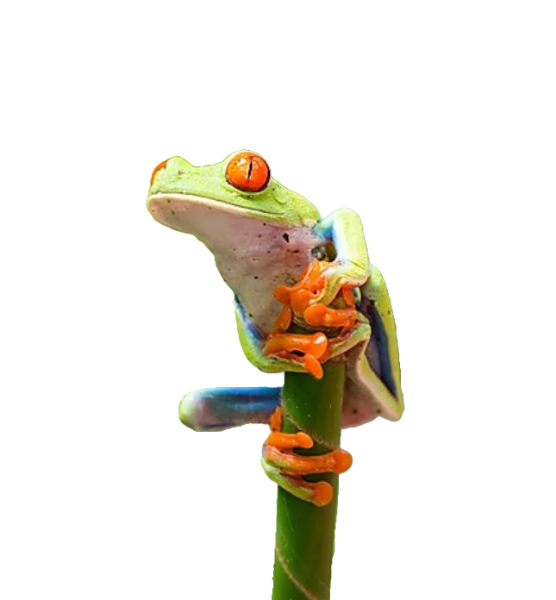
\includegraphics[width=0.75\linewidth]{images/kikker_voorkant.png}
\bigskip
\bigskip

%% Print the name of the author.
{\makeatletter
%\largetitlefont\Large\bfseries\@author
\largetitlestyle\fontsize{26}{26}\selectfont\@author
\makeatother}

\vspace{1cm}

\fontsize{15}{15} \tudsffamily \today

\vfill

\begin{table}[H]
    \Large
    \centering
    \begin{tabular}{l|l}
    R. Copier & 4354095
    \end{tabular}
\end{table}




%\centering{
\includegraphics{cover/logo_black}}


\end{center}

\begin{tikzpicture}[remember picture, overlay]
    \node at (current page.south)[anchor=south,inner sep=0pt]{
        
\includegraphics{cover/logo_black}
    };
\end{tikzpicture}


\end{titlepage}

% \chapter{Abstract}


\textbf{Keywords:}

% \input{chapters/summary.tex}
\chapter{Preface}\label{ch:preface}



\newpage
\thispagestyle{plain} % empty
\mbox{}

\chapter{Abstract}


\textbf{Keywords:}


\newpage
\thispagestyle{plain} % empty
\mbox{}

% \newgeometry{top=5mm, bottom=22mm}
\setcounter{tocdepth}{2}
{\small\tableofcontents}
% \restoregeometry
%\input{chapters/Glossary}
%\printnomenclature


\mainmatter
\chapter{Introduction}\label{ch:introduction}
\section{Reversible adhesion: current challenges}\label{sec:current_challenges}
\section{Existing solutions}\label{sec:existing solutions}
\section{Bio inspired approach to reversible adhesion}\label{sec:bio_inspired_approach}
\subsection{Tree frog adhesive mechanisms}\label{sec:tree_frog_adhesion}
\subsubsection{Morphology}
\qquad Tree frogs use the so-called mechanism of wet adhesion to adhere to surfaces in their living environment. Animals using wet adhesion use fluids to increase their adhesional performance and tree frogs do so by secreting watery mucus. The exact functionality of the mucus secreted by tree frogs is not yet clear. Studies show that both viscous forces and surface tension are likely to contribute to the adhesional performance of the tree frog \cite{hanna1991adhesion}. Adhesional performance is furthermore dependent on the compliance of the adhesional pads. Adhesional pad compliance is relevant for all animal that make use of reversible adhesion. The compliance of the adhesional pads is dependent on morphological properties of the pads used by animals to adhere to a surface. The morphological properties of the digital digits of the different species of tree frogs described in literature are very similar. In fact, it is usually not possible to identify the family from the appearance of the toe pads \cite{barnes2011elastic}. The morphological properties described below are from observations on the \textit{Litoria Caerulea White} by Scholz et al. and by Barnes et al. \cite{scholz2009ultrastructure,barnes2011elastic} and on the \textit{Osteopilus Septentrionalis} by Hanna et al. \cite{hanna1991adhesion}.\\

\qquad A study by Langowski et al.\cite{langowski2018force} reveals the morphological properties of the \textit{Hyla Cinerea}. This study does not only analyze the epidermal properties but also gives insight in the dermal structure of the tree frog digits. The morphological properties of the rock  frog \textit{Staurois Parvus} described by Drotlef et al. \cite{drotlef2015morphological} are slightly different from the properties of the \textit{Hyla Cinerea}.\\ 

% Epidermal structure, over de zeskantige cellen
\qquad The specialised adhesive pad epithelium of the \textit{Hyla Cinerea} is 10- to 15 \textmu m thick and delineated from the normal skin by distinct grooves. The epidermis consists of four to six layers of columnar epithelial cells. The outermost layer is non-living and consists out a polygonal epithelial cells. Most of these are hexagonal but pentagonal, heptagonal an octagonal formed epithelial cells are also observed. The structure of the second cell layer is very similar to the structure of the outer cell layer. This layer will become the outer layer when the first layer has worn of. The epithelial cells contain keratin fibrils with are oriented at an angle to the surface. For both tree frogs and rock frogs the fibrillar structures in the epithelial cells are distally pointed.\\ 

\qquad The amount of angling varies between species: for some species the fibrillar structure is almost normal tot the surface while for other species like the \textit{Hyla Cinerea} as described by Langowski et al.\cite{langowski2018force}, the fibrillar structures are more angled as is visible in Figure \ref{fig:epidermal_structures_all}. The nanopillars on top of the epithelial cells are formed from the end of these keratin filaments and (partly) fill these structures. The presence of the keratin filaments increases the stiffness of and the wear resistance of the epithelial cells and the nanopillars on top of these and the angling of the keratin filaments gives the adhesive pad directional dependent properties.\\ 

% over de afmetingen van de epithelial cells en channels ertussen
\qquad The epithelial cells have a diameter of 13 \textmu m. A network of channels exists between the epithelial cells. This channel network follows the hexagonal pattern of the epithelial cells for the tree frogs. The adhesive pads of the rock frogs however has more stratified channels which form a shorter route to the channel running around the toe pads. The channels between the epithelial cells for both tree frogs and rock frogs have a width of about 1-2 \textmu m and are about 10 \textmu m in depth. The channel surrounding the toe pad not only functions in drainage of excess water from the pad but is also ideally placed to channel fluid around rather than under the pad.

\begin{figure}[h!]
     \begin{subfigure}{0.45\textwidth}
         \centering
         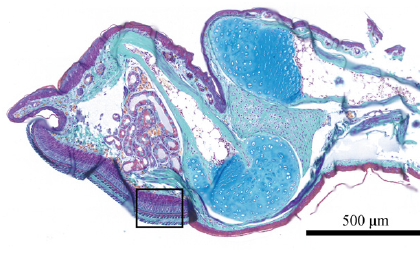
\includegraphics[width=\linewidth, height=5.5cm, angle=0]{images/epidermal structure/epidermis_langowski_1.png}
         \caption{}
         \label{fig:toe_pad_section}
     \end{subfigure}
     \hfill
     \begin{subfigure}{0.45\textwidth}
         \centering
         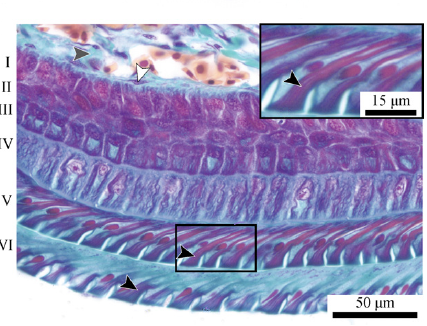
\includegraphics[width=\linewidth, height=5.5cm, angle=0]{images/epidermal structure/epidermis_langowski_2.png}
         \caption{}
         \label{fig:epidermis_different_levels}
     \end{subfigure}
     \hfill
    \caption{Pictures from the paper by Langowski et al. \cite{langowski2018force} which show the epidermal structure to the level of the epithelial cells. (a) A mid-sagittal section of a digital pad of the Hyla Cinerea. (b) A magnified view of the ventral epidermis. The cellular layers are visible and numbered with the numbers \rom{1}-\rom{6}. The fibrillar structure has a reddish colour and is better visible in the magnified view in the top right of the image. The black arrows point to the fibrillar structure in the epithelial cells, the white arrows to the reticular cells and the grey arrows point to the reticular connective tissue.}
    \label{fig:epidermal_structures_all}
\end{figure}


% over de nanopillars 
\qquad The surfaces of the epithelial cells are covered with closely packed columnar nanopillars. The dimensions of these pillars vary between species and measures 200 nm to 350 nm in diameter for the frog species \textit{Osteopilus Septentrionalis} and \textit{Staurois Parvus}. The height of the nanopillars for these frogs is 300 - 500 nm which gives the pillars an aspect ratio between 1 and 2. The nanopillars of the \textit{Litoria Caerulea} are smaller with a diameter and height of approximately 22 nm.\\ 

\qquad The nanopillars as visible in Figure \ref{fig:nanopillars} do contribute to the frictional and adhesive properties of the adhesive pads. The most probable mechanism for this performance enhancement is that the nanopillars allow for close conformation to surface irregularities. Just as the epithelial cells, but at a much smaller length scale. This close conformation activates Van der Waals forces and increases capillary forces through thinning of the fluid layer between adhesive pad and substrate. The close surface conformation is mainly caused by by the presence of the grooves surrounding each nanopillar and by the compliance of the pillars caused by the low stiffness of the pillars and by their aspect ration which allows them to bend easily. The nanopillars mainly effect the frictional forces which come close to dry frictional forces due to the close contact made between the adhesive pad and surface. Their role in capillary forces is expected to be much less since such forces are generated by the air-water interface around the edge of the pad \cite{ernst1973digital}.\\

\qquad The nanopillars each have a slight depression or ‘dimple’ on top of each pillar. This dimple has a depth of approximately 6-8 nm and the edges of these dimples are interrupted with one or two channels connecting the dimple with the surrounding space between the nanopillars. Between the nanopillars are channels. These channels form a part of the channel network on the adhesive pads which drains excess water from the pads and acts as a reserve to make capillary adhesion possible on dry surfaces. The channels connecting the dimples with the channels around the nanopillars extend this channel network.\\ 

\begin{figure}[h!] 
\begin{subfigure}{0.48\textwidth}
    \centering
    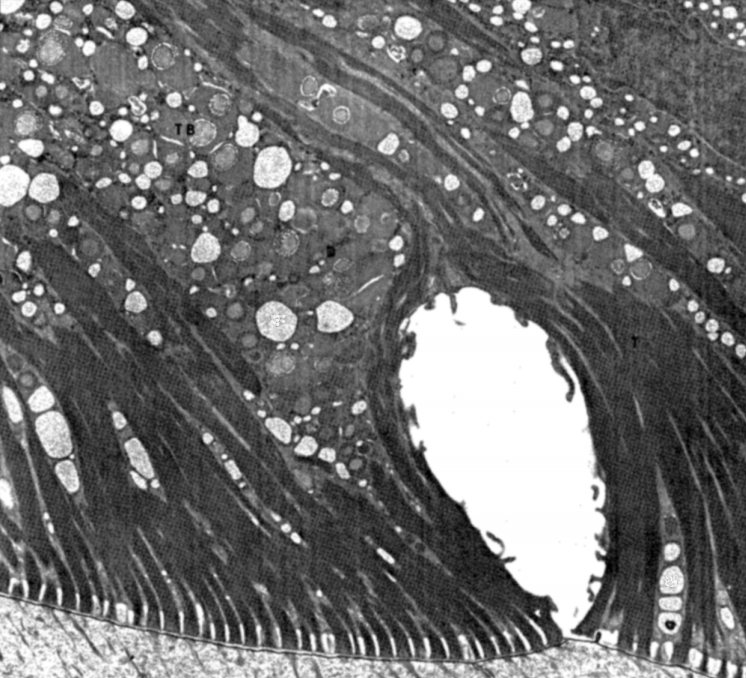
\includegraphics[width=\linewidth, height=6cm, angle=0]{images/epidermal structure/epithelial_cells_and_nanopillars_ernst.PNG}
    \caption{}
    \label{}
\end{subfigure}
\hfill
\begin{subfigure}{0.48\textwidth}
    \centering
    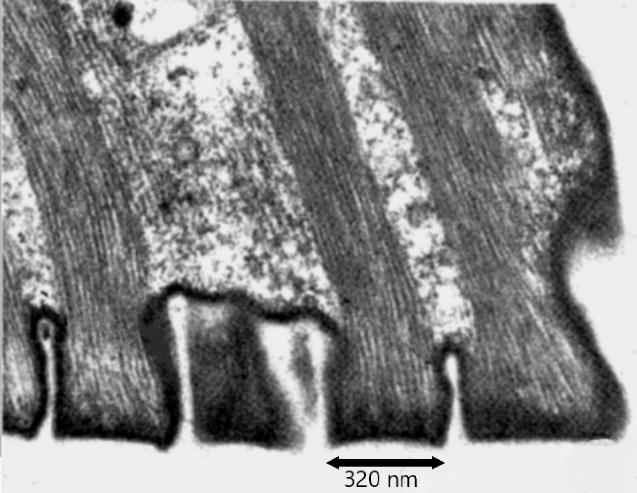
\includegraphics[width=\linewidth, height=6cm, angle=0]{images/epidermal structure/nanopillars_ernst.PNG}
    \caption{}
    \label{}
\end{subfigure}
 \caption{Pictures from the paper by Ernst et al. which show the structures of the adhesive pads of the Hyla cinerea \cite{ernst1973digital}. (a) Epithelial cells on which multiple nanopillars are visible. The dark lines visible are the keratin fibres which originate in the epithelial cells and run up to the surfaces of the nanopillars. (b) Close-up of the nanopillars with a more detailed view on the keratin fibres. The width of one nanopillar as depicted above is an estimation based on the data provided by Ernst et al.}
 \label{fig:nanopillars}
\end{figure}

% over de ventral collogen layer
\qquad The epidermal layer is supported by the dermal structure of the toe digit. In Figure \ref{fig:epidermis_different_levels} are the reticular cells visible. The cells in this layer connect the epidermal structure with the higher level dermal structure, the dermal stratum spongiosum. The amount of keratin fibres reduces with the depth of the epidermis. This confirms the stiffness measurements described above.\\ 

\qquad Scholz et al. describe a decrease in the density of the cytoskeletal elements in the epidermal structure. They describe that the diameters of the pores in the epithelial cell structure are smaller towards the outer surface of the cell. In the deeper cell layers they describe a lose lattice of fibrillar material. This also explains why the outer epidermal structure has a higher stiffness than the underlying material. From the literature available it can be concluded tree frog adhesive pas have a thin but slightly harder ‘skin’, with a Young’s modulus equivalent to silicon rubber, covering a soft gel-like structure.\\ 

\qquad This gel-like structure, the dermal stratum spongoisum has a dense network of capillaries. This capillary network is similar to the blood sinuses that occur beneath the hairy adhesive pads of gecko's and are thought to act as a hydrostatic skeleton maintaining pressure on the scansors that hold the adhesive setae. When the digit is brought in contact with a surface, the phalanx in the digit presses down on the structure between the phalanx and the epidermis. This increases the pressure in the dermal structure above the epidermis and presses the pad on the substrate. It is possible that the tree frog uses its capillary network in the stratum spongiosum in a similar way.\\ 

\begin{figure}[!ht]
    \centering
    \raisebox{-0.5\height}{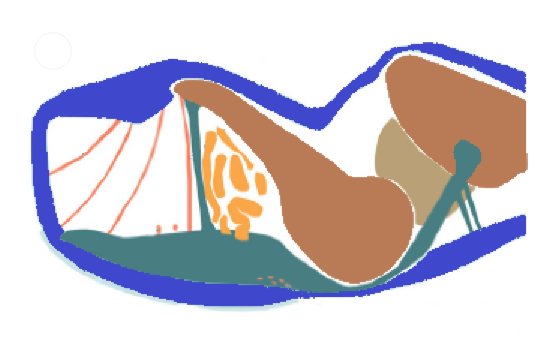
\includegraphics[width=0.45\linewidth, height=5.5cm, angle=0]{images/epidermal structure/schematic_view_voorlopig.PNG}}
    \hspace*{.2in}
    \begin{tabular}{p{0.3cm} p{4cm}}
    \mycbox{blueviolet} & Apical dermis/Basal epidermis\\ 
    \mycbox{lightblue} & Adhesive epidermis\\
    \mycbox{collagen_color} & Collagen material\\ 
    \mycbox{glands_color} & Mucus glands\\
    \mycbox{phalanx_color} & Distal and middle phalanx\\ 
    \mycbox{intercalary_color} & Intercalary element\\
    \mycbox{muscle_color} & Muscle fibers\\
    \end{tabular}
    \captionlistentry[table]{A table beside a figure}
    %\captionsetup{labelformat=andtable}
    \caption{Schematic representation of the dermal structure. This figure is derived from the paper form Langowski et al.\cite{langowski2018force}.}
    \label{fig:dermal_structure}
\end{figure}


\qquad The collagen layer is well described in the work of Langowski et al. This layer fills the space between the epidermis, the gland space and runs below the base of the distal phalanx. Proximal to this base, it converges and connects to the side arms of the collateral ligaments. The collagen ridges gradually flatten and and vanish towards the distal end of the pad. The collagen layer has a fibrous structure and the fibres are oriented along the distal-proximal axis. The collagen layer below the gland space is separated in longitudinal ridges. Mucus ducts and blood vessels occupy the space in the troughs between the ridges. The ridges are not visible in the proximal part of the collagen layer.\\

\qquad The ridges in the collagen layer compensate for the loss in tensile strength caused by the the mucus ducts which perforate the collagen layer and with that, weaken its structural integrity. This is also confirmed in the paper by Langowski et al. in which is shown that the ridges are oriented along the trajectories of the maximum stresses along the ventral surface of the adhesive pad. It is also quite probable that the collagen layer has a lower stiffness in the transverse direction than in the longitudinal direction. The stresses for which the collagen layer is optimally designed occur when the ventral surface is loaded by proximal shear along the ventral pad surface.\\ 
    
\qquad The dermal pad structure is divided in two parts by a septum that runs from the distal tip of the phalanx towards the ventral epidermis. In the distal compartment the dermal stratum spongiosum can be found which has a very soft structure due to lymph filled spaces that are present in this compartment. Furthermore, there are two types of muscle fibres present in the space distal to the collagenous septum: in Figure \ref{fig:dermal_structure} a group of muscle fibres is visible which is oriented in ventral-dorsal direction. Another group of cross-lateral muscle fibres is also visible in Figure \ref{fig:dermal_structure}. There are two distinct thick muscle fibres that run from the tip of the distal phalanx to the ventral collagen layer. Although most muscle fibers are located in the distal lymph space, there is also one group of cross-lateral muscle fibers proximal to the collagenous septum. These muscle fibres are embedded in the collagen layer discussed above.\\ 
\qquad The dermal structure proximal to the collagenous septum contains numerous mucus glands. The glands in this gland space are all connected to the ventral pad surface via mucus ducts that traverse the dermal structure. These ducts lie in the troughs between the ridges of the collagen layer discussed above.\\

\subsubsection{Behavioural adaptions}\label{sec:intro_spreading}
\qquad A study performed by Endlein et al. \cite{endlein2013sticking} shows that tree frogs actively change their position when higher adhesional forces are required. The tree frogs change their position to a sprawled position by extending their legs laterally. This reduces the contact angle between pads and substrate and increases the lateral forces between at the contact interface. This spreading is visible in Figure \ref{fig:tree_frog_limb_spreading}. 

\begin{figure}[h!] 
\begin{subfigure}{0.32\textwidth}
    \centering
    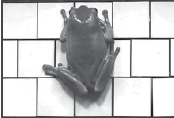
\includegraphics[width=\linewidth, height=4cm, angle=0]{images/limb spreading/Tree_frog_spread_rest_endlein2013sticking.png}
    \caption{}
    \label{fig:limb_spreading_rest}
\end{subfigure}
\hfill
\begin{subfigure}{0.32\textwidth}
    \centering
    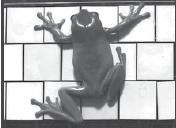
\includegraphics[width=\linewidth, height=4cm, angle=0]{images/limb spreading/Tree_frog_first_spread_endlein2013sticking.png}
    \caption{}
    \label{fig:limb_spreading_first_spread}
\end{subfigure}
\begin{subfigure}{0.32\textwidth}
    \centering
    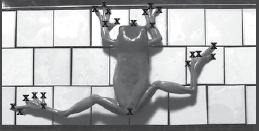
\includegraphics[width=\linewidth, height=4cm, angle=0]{images/limb spreading/Tree_frog_second_spread_endlein2013sticking.png}
    \caption{}
    \label{fig:limb_spreading_second_spread}
\end{subfigure}
  \caption{Stages in the limb spreading of the tree frog on inclined surfaces \cite{endlein2013sticking}. (a) The initial position of the resting frog. (b) The first spread of the frog. (c) The second spread of the frog.}
  \label{fig:tree_frog_limb_spreading}
\end{figure}

\qquad There are two stages visible in this limb spreading: the frog first spreads its limbs when adhesional performance in the resting position is insufficient (Figure \ref{fig:limb_spreading_first_spread}). The frog spreads its limbs even further when the adhesional performance in the first spread is insufficient (Figure \ref{fig:limb_spreading_second_spread}). The impact of this spreading behaviour is further described in Section \ref{sec:behavioral analysis}. 

\qquad The magnitude of the forces involved in the proximal pulling are visible in Figure \ref{fig:mag_pulling}. This figure shows that the magnitude of the proximal pulling force has a maximum value of approximately one-fifth of the body weight. The large variation visible in the results of Endlein et al. however, does not allow for an accurate estimation of the pulling force magnitude. 

\begin{figure}
    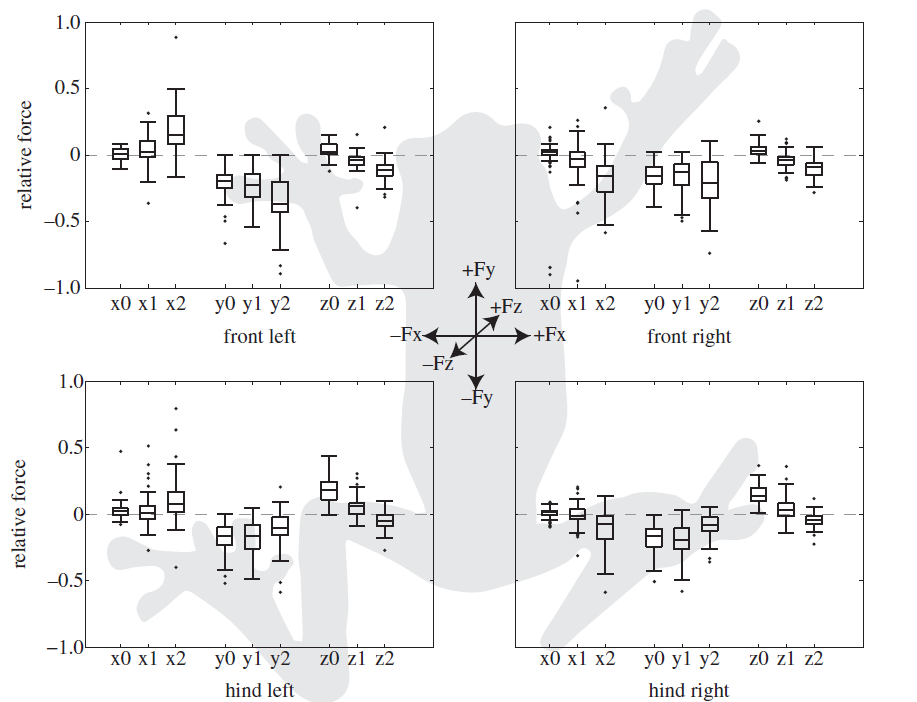
\includegraphics[width=0.65\linewidth, height=7cm, angle=0]{images/limb spreading/work_endlein.PNG}
    \caption{Relative force as force per body weight generated at the interface of the individual limbs. The resting position, first and second spread is indicated by the indexes 0, 1 and 2 respectively.}
    \label{fig:mag_pulling}
\end{figure}







\subsubsection{Bio material properties}\label{sec:bio_material_properties}
The epidermal structure of the tree frog is composed of different bio-materials. The exact composition this structure is known to be dependent on the age of the animal \cite{barnes2011elastic} and it furthermore likely to be dependent on species and living environment as it is for other animals \cite{peng2016microstructure}. The adhesional performance of the animal is dependent on the mechanical properties of the adhesive pads. Actual measurements of these properties are described in studies by Barnes et al. and in work from Scholz et al. \cite{barnes2005mechanical,scholz2009ultrastructure,barnes2011elastic,barnes2013comparative,kappl2016nanoscale}. The results from the stiffness measurements are visible in Table \ref{tab:experiments_literature}. The content of this table matches the content published by Langowski et al. \cite{langowski2018tree}. The Young's modulus of the adhesive pads is found to be inversely proportional to the indentation depth. This behaviour makes the toe epidermis self-adaptive to an applied load. The pads show pure elastic deformation indented more than $200 \mu m$ \cite{barnes2011elastic}. Furthermore, the toe pad epithelium is found to be stiffer than the dermal material directly under the epithelium. 


\begin{table}[h!]
\hspace*{-1cm}\begin{tabular}{p{2cm}|p{2cm}|p{1.5cm}|p{1.5cm}|p{1.5cm}|p{1.5cm}|p{1.5cm}|p{1.5cm}|p{2cm}}
Species & Setup & Diameter indentor [$\mu m$] & Indentation depth [$\mu m$]  & Frequency [Hz] & Indentation velocity [$\mu m$] & Stiffness mean value [kPa] & Work of adhesion [$J/m^2$] & Source\\ 
\hline
Litoria Caerulea & Whole frog with restricted limbs, temporally anesthetized & & 1.6 & 1-2 & 3.2-6.4 & 5.7e3 & & Scholz 2009\\
\hline
Litoria caerulea & & & 50 - 350 & & & 12 & & Barnes 2005\\
\hline
Litoria Caerulea & Whole frog with restricted limbs, temporally anesthetized & 1500 & 350 & 1/35, 5 s relaxation time & 23 & 4.45 & 0.08 & Barnes 2011 \\
\hline
Litoria Caerulea & Toes removed from frogs & 0.04 & 0.2 & 0.5 & & 33.5& & Barnes 2013\\
\hline
Rhacophorus Prominanus & Toes removed from frogs & 0.04 & 0.2 & 0.5 & & 28.7 &  & Barnes 2013  
\end{tabular}\hspace*{-1cm}
\caption{Setup and results from indentation experiments described in literature}
\label{tab:experiments_literature}
\end{table}


\qquad In Table \ref{tab:experiments_literature} is visible that the stiffness values found for the experiments described by Scholz are much higher than the values found in the studies of Barnes et al. In the paper published by Barnes in 2011, the author ascribes the the higher measured stiffness in the study by Scholz et al. to the the difference in indentation depth between the experiment carried out by Scholz and the experiment carried out by Barnes in 2011. The experiments by Barnes et al. from 2013 however, use a similar technique and indentation depth as used by Scholz et al. in 2009 and still report much lower values for the stiffness than reported by Scholz et al. Possible other explanations between this difference in measured stiffness are:
 \begin{itemize}
     \item The indentation frequency used in the experiments of Scholz is higher. This can allow viscoelastic effects to play a role. The stiffness of most viscoelastic materials increases with an increase in loading frequency. 
     \item The experiment by Barnes et al. from 2013 involves tree frog toes that are separated from the animal while the experiment by Scholz et al. involves living tree frogs. Measurements on living tissue are more sensitivity to animal induced distortions such as the animals heart beat. 
     \item For the study by Barnes et al., the cut-off limbs were placed in a Ringer's solution. This solution can soften the epithelial tissue, especially the outer layer of the cellular layers. This effect can play a significant role since the indentation depth is relative small in the experiment by Barnes et al. from 2013. 
     \item It is known that the stiffness of epithelial material increases with the age of the tree frog \cite{barnes2011elastic}. A difference in age between the frogs used by Barnes and Scholz could play a role in the difference in measured stiffness between these two studies. 
     \item The mathematical models to calculate the stiffness from the indentation data differs between the studies under consideration. Barnes describes a modified version of the Hertz contact model while Scholz has uses a force-indentation model form Oliver and Parr. Both models can be used to calculate stiffness values but it is possible that these models produce different results for similar input data. 
 \end{itemize}
 
 \qquad As a consequence of the relatively large difference between the reported values of the stiffness of the adhesive pads, the stiffness of these pads needs to based on a choice of one of the values reported in literature while neglecting the other. The stiffness values reported by Barnes et al. are considered the most reliable because:
 \begin{itemize}
     \item The stiffness values reported in the three individual papers by Barnes et al. are all in the same range while each individual paper reports another theoretical model used to calculate the stiffness values from the raw measured data.
     \item The paper published in 2011 describes that the tested samples where tested at such frequency to eliminate viscoelastic effects. 
     \item The paper published in 2013 gives the stiffness of the epithelial layer of two different frog species. The measured values are of the same order of magnitude.
 \end{itemize}

\qquad The stiffness measurements from the studies of Barnes et al. give an order of magnitude for the stiffness of the epithelial layer of the tree frog. These stiffness measurements however, need to approached carefully:
\begin{itemize}
    \item The results of the stiffness measurements obtained with the smallest indentation depths($0.2 \mu m$) are expected by be very sensitive to variations in on the surface of the epithelial layer. The surface of the epithelial layer consists of nanopillars as is visible in Figure \ref{fig:nanopillars}. An indentation measure between two nanopillars is expected to produce a very different results than a similar measurement on the surface of a pillar.
    \item The adhesive pads are expected to have a direction dependent stiffness due to the fibrillar internal structure. The stiffness measured with an indentation measurement does not apply an tensile load on the internal fibers. The stiffness measured in an experiment in which the internal fibers are loaded in tension is therefore expected to be significantly higher. The stiffness values reported by Barnes et al. are expected to be in the range of the stiffness of the material surrounding the fibers. The stiffness of this material is expected to be of significantly lower stiffness than the fiber material. 
    \item The epithelial cells are partially filled with cytoplasm. This liquid will increase the compliance of the epithelial cell, especially when the indentation frequency is low enough to prevent viscoelastic effects.
\end{itemize}

\qquad Figure \ref{fig:epithelial_cell_components} shows the most important components of an epithelial cell. This Figure a modified version off a figure from the work of Langowski et al. \cite{langowski2018force}. The nucleus visible is the figure is relatively large but is not expected to significantly contribute to the mechanical properties of the cell and therefore neglected.

\begin{figure}
    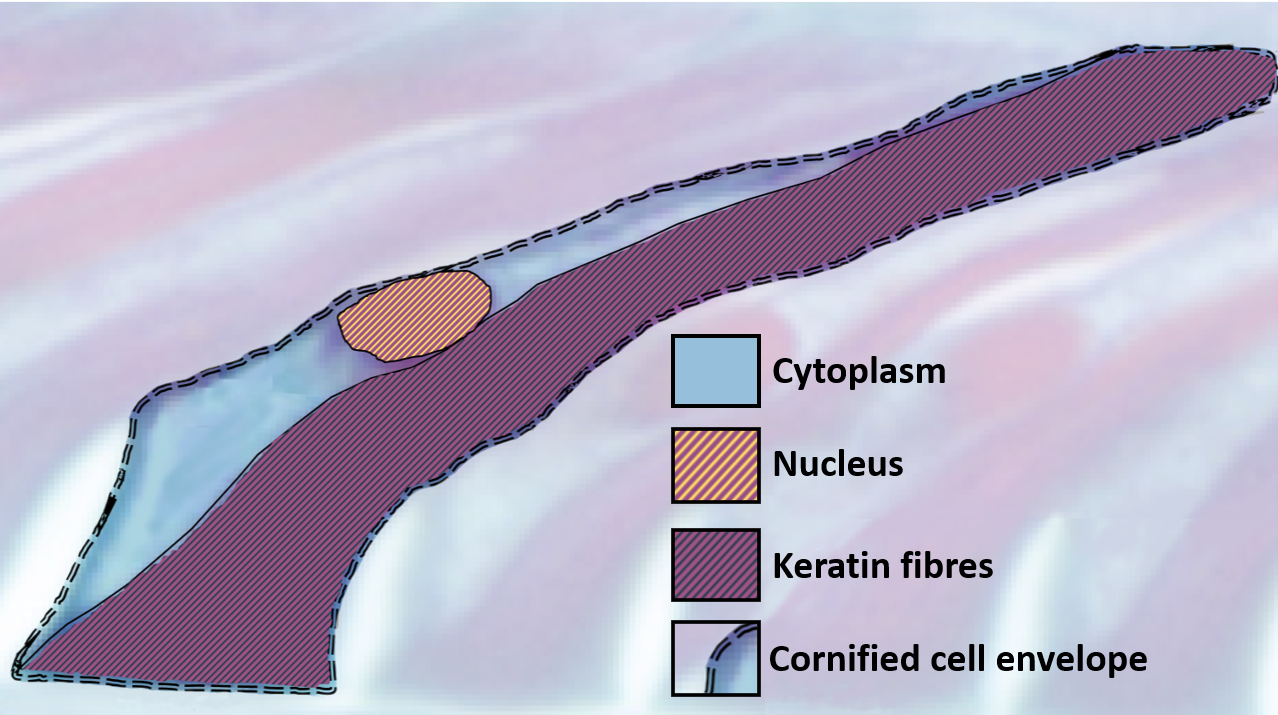
\includegraphics[width=0.60\linewidth, height=5.5cm, angle=0]{images/epidermal structure/cell_langowski_modified.PNG}
    \caption{Epithelial cell with the most important cell components.}
    \label{fig:epithelial_cell_components}
\end{figure}

 
\qquad The stiffness measurements on the tree frog can be compared to other stiffness measurements performed on animal tissue. The mechanical properties of animal tissue depend on the type of protein and on the level of hydration. One of the most frequent proteins is collagen. The fibers in the tree frog epithelial layer are composed of keratin which has a higher stiffness than collagen.\\
 
\qquad The stiffness for animal keratin in literature are given in Table \ref{tab:animal_keratin}. The animal keratin found in mammals can be classified as alpha or helical keratin while the keratin found in birds and reptiles can be classified as beta or pleated-sheet keratin \cite{bonser2000young}. The elastic properties of keratin in birds and reptiles are therefore considered more representative for the keratin properties of the tree frog. In the table below is also visible that the elastic moduli of the birds claw, the birds feathers and the gecko setae are very similar.\\

  
\begin{table}[h!]
\centering
\begin{tabular}{p{3cm}|p{2.5cm}|p{1cm}}
Origin                          & Elastic modulus [GPa]& Source                 \\
\hline
Sheep wool                      & 7-47              & \cite{simpson196551}\\
Human keratinocyte cytoskeleton & 1.2e-4 3.4e-4     & \cite{lulevich2010single}\\
Birds claw                      & 1.84              & \cite{bonser2000young}\\
Birds feathers                  & 2-5               & \cite{cameron2003young}\\
Gecko setae                     & 1.5               & \cite{peattie2007ancestrally}\\
Horse-hoof                      & 0.41 - 14.6       & \cite{bertram1987functional}
\end{tabular}
\caption{Stiffness values for animal and human keratin. The lower three rows give the stiffness values of pleated sheet keratin and are thus most relevant.}
\label{tab:animal_keratin}
\end{table}
  

\qquad The keratin fibers are embedded in connective tissue. Connective tissue typically has a lower stiffness than keratin but the exact composition of the connective tissue is not described in literature. Common connective tissue in bio-structures are collagen and elastin. The material properties of collagen are listed in Table \ref{tab:animal_collagen}. The collagen material properties are slightly lower but in the same range as the keratin material properties. This can be caused by the highly directional properties of the the tissues used to determine these stiffness values. Such directional properties are not visible in the material between the keratin fibers and above and below these fibers in the epithelial cell. The elastic properties of elastin indicate a much lower stiffness than the stiffness of collagen.\\ 

\begin{table}[h!]
\centering
\begin{tabular}{p{3cm}|p{2.5cm}|p{1cm}}
Origin                               & Elastic modulus [GPa] & Source                 \\
\hline
Collagen, rat tail tendon            & 3.75                  &\cite{wenger2007mechanical}\\
Collagen, bovine Achilles tendon     & 9.0                   &\cite{harley1977phonons}\\
Collagen, rat tail tendon            & 0.1 -0.36             &\cite{dutov2016measurement}\\  
Collagen, bovine Achilles tendon     & 0.002 - 0.2           &\cite{grant2009tuning}\\
Bovine elastin                       & 0.00041               &\cite{aaron1981elastin}\\
Bovine elastin                       & 0.0011                &\cite{gosline2002elastic}
\end{tabular}
\caption{Stiffness values for animal connective tissue.}
\label{tab:animal_collagen}
\end{table}


\qquad The stiffness values found in literature for collagen are relative close to the stiffness values found for keratin. The stiffness of these bio-materials however can be severely influenced by the degree of hydration. Grant et al. describes a range of $2-200 MPa$ for bovine collagen in varying solution conditions \cite{grant2009tuning} and Bertram et al. \cite{bertram1987functional} describes that the stiffness of horse-hoof keratin can be varied over a range of $0.41 - 14.6 GPa$  depending on the hydration of the material.\\ 

\qquad The relatively high stiffness measurements on hairs, claws, feathers and setae as visible in Table \ref{tab:animal_keratin} are all obtained from dead and relatively dry material. The stiffness of these materials is much higher than the stiffness of living keratinous material like keratinocytes as also visible in Table \ref{tab:animal_keratin}. These keratinocytes are much better hydrated than the dead keratinous materials. Furthermore, it should be noted that keratinocytes are living cells which also contain other cell elements which are most likely not as stiff as the keratinous elements in these cells. The stiffness of pure keratinous fibers is therefore expected to be in the range of $1-10 GPa$.\\ 

\qquad The exact composition of the connective tissue between the fibers is not reported in literature. Based on the stiffness values visible in Table \ref{tab:animal_collagen}, the stiffness of the connective tissue between the keratin fibers is most probable somewhere in between the stiffness values reported for collagen and elastin. Furthermore, the connective tissue in the epithelial cells is well hydrated. The effective stiffness of the connective tissue is therefore estimated at a range of $1-10 MPa$.\\

\qquad The most superficial layer of the cell epidermis outer epithelial layer of the adhesive pads is argued to have a relatively high stiffness \cite{nakano2016light}. This $10 nm$ thick layer is composed of insoluble proteins and its stiffness is most probable in the range of the keratinous cell elements.\\




% je kunt nog de literatuur in om strain stiffening voor keratine op te zoeken en daar dan ook weer een model van maken-is wel zo netjes



\section{Wet adhesive mechanism: theory and application}\label{sec:adhesive_theories}
% hier kunnen we dus ingaan op de bestaande theorien om de functie van de elementen in de poot van de kikker uit te leggen
% we doen de informatie die ik al opgezocht heb voor de literatuurstudie en vatten dit samen:
% -capillary forces en andere mechanisms die een rol spelen voor de 'natte' component
% - mechanismen die een rol spelen voor de droge adhesie
\subsection{Capillary forces}
The Laplace capillary force is defined as visible in Equation \ref{eq:laplace_capillary_general} \cite{laplace1799traite}. With $\gamma$ for the surface tension, $\Delta P$ for the pressure difference and $R_1$ and $R_2$ for the radii of the two contact surfaces that are involved in the contact. When these radii become very large, the liquid volume needed between the two surfaces is reduced to almost zero, increasing the value of the capillary pressure difference $\Delta P$. The minimum amount of adhesive liquid between two surfaces is dependent on the degree of roughness of these surfaces \cite{qian2006scaling}. The limit of the pad-substrate gap size reduction is at the critical length for which the fluid itself would fail due to cavitation. Very thin fluid layers can also lead to unstable spreading and shrinking of the fluid layer \cite{yi2009dynamic} and are thus undesirable for the generation of stable adhesive forces.\\ 
\begin{equation}
    \Delta P = - \gamma (\frac{1}{R_1} + \frac{1}{R_2})
    \label{eq:laplace_capillary_general}
\end{equation}

\qquad The Another factor of influence in capillary adhesion is the contact angle. An increase in the contact angle generally results in an increase in the required liquid volume to establish full contact and with that reduce adhesion \cite{qian2006scaling}. It is found that an adhesive pad will always achieve the maximum adhesive strength and robustness when the effective contact angle is smaller than a critical value \cite{su2009concave}. For flat contact surfaces, this critical angle is around 30 degrees \cite{orchard2012influence}. Su et al. discovered that a concave pad geometry transfers the contact angle to a smaller contact angle. This concave geometry increases the critical contact angle to a value of 45 degrees.\\

\qquad The role of the surface tension is still under discussion. According to Smith et al.  \cite{smith2006adhesion} the magnitude of the capillary forces can be explained by a presence of a surface tension based force \cite{peng2016microstructure}.  This capillary force depends on the amount of liquid bridges formed, the volume of the individual droplets and on the contact angles from the droplets to the substrate and to the adhesive pad. Others however state that the tenacities measured for tree frogs are in the same range as capillary forces measured between two glass plates \cite{langowski2018tree}. This suggests that there is only one continuous liquid meniscus between the two surfaces \cite{scholz2009ultrastructure} which makes that the surface tension contribution can not be considered as significant since it is dependent on the amount of liquid bridges formed.\\

\qquad The secretion fluids are an emulsion of hydrophilic and hydrophobic components. This emulsion is able to stick well to hydrophilic and hydrophobic surfaces \cite{langowski2018tree}. The hydrophobic or hydrophilic pad properties can have a severe influence on the adhesive performance for large contact angles. For contact angles below the critical value of 30 degrees the hydrophobic or hydrophilic surface properties do not severely change the adhesive pad properties \cite{orchard2012influence}.\\

\subsection{Van der Waals forces}
\qquad Although capillary forces are considered the main adhesional mechanism for tree frogs, there are also measurements that indicate the existence of dry contact interaction between adhesional pads and substrate \cite{kappl2016nanoscale}. These dry contacts do most likely occur on epithelial cell borders and at the location of nanopillars that come close enough to the substrate to establish dry contact. Dry contact allows Van der Waals forces to play a role. These contact forces can also play a role in very thin liquid layers though molecular ordering and interaction in the fluid \cite{federle2004biomechanics}. Dry contact interaction through Van der Waals forces is furthermore dependent on the temperature, ambient humidity and on the sliding velocity for sliding contacts.\\ 

\qquad The forces involved in dry contact interaction can be calculated with the Kendall equation which represents a peeling model for sticky rubber tape as visible in Equation \ref{eq:Kendall_equation}. This equation calculates the work of adhesion $W_a$ with the applied force $F$, the peeling angle $\alpha$, $d$ for the width of the tape with a Young's modulus $E$. According to this equation, friction forces are high for small values for $\alpha$. The force scales with the width of the tape because the peeling stress concentrations are found on the edges of the tape under peeling stress. This contact angle dependence is also observed in the previous section about capillary adhesion. A low contact angle can also cause crack healing to occur for critical peeling force values.\\
\begin{equation}
    W_a = F(1-cos(\alpha)) + \frac{F^2}{2dE}
    \label{eq:Kendall_equation}
\end{equation}

\subsection{Tree frog inspired applications}\label{sec:tree_frog_applications}
\qquad The work by Xue et al. describes an application of an fiber re-enforced material inspired on the toe pads of tree frogs. This work describes the difference in stress the distribution in the composite material between a fiber re-enforced material in which the fibers and the base material are properly attached to each other and a material in which the fibers and the base material are not bound to each other. The adhesional performance of both materials is evaluated with a measurement of the vertical pull-of force needed to release the material from a substrate. The materials where compressed into the substrate prior to the pull-of force measurement.\\

\qquad The results obtained by Xue show that the stress in the composite in which the base material and the fibers are properly bound has a much lower maximum value. Furthermore, the maximum stress is not located at the edge of the geometry but can be found at a certain distance(1-2 rows of pillars from the edge) from the material edge. A composite material in which the fibers are not bound to the base material has a maximum stress on the edge of the geometry as is also the case for homogeneous materials. The stress distributions for the material with the well-bound and the loose fibers are visible in Figure \ref{fig:Xue_model_1} and \ref{fig:Xue_model_2} respectively.\\ 

\begin{figure}[h!] 
    \begin{subfigure}{0.49\textwidth}
    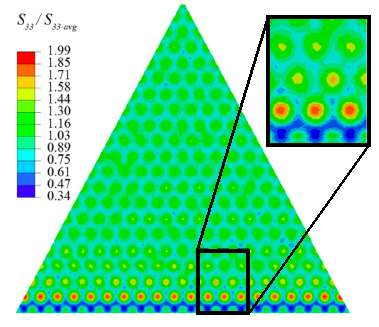
\includegraphics[width=\linewidth, height=6cm, angle=0]{images/Xue_work/Xue_model_internal_bounding.png}
    \caption{}
    \label{fig:Xue_model_1}
    \end{subfigure}
        \hfill
    \begin{subfigure}{0.49\textwidth}
    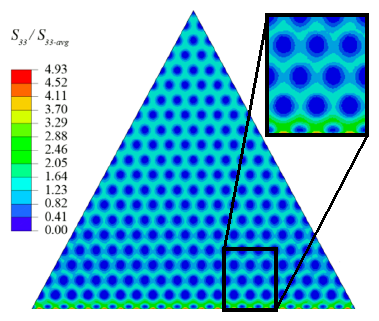
\includegraphics[width=\linewidth, height=6cm, angle=0]{images/Xue_work/Xue_model_internal_loose.png}
    \caption{}
    \label{fig:Xue_model_2}
    \end{subfigure}
    \caption{Pictures from the modeling work by Xue et al. The stress distribution in (a) is the result of the internal bounding between the fibers and the base material. The stress distribution in (b) has a larger stress peak on the edge of the geometry. This is due to the absence of internal bounding between the fibers and the base material. It should be noted that only the $S_{33}$ component is taken into account.}
    \label{fig:all_images_Xue}
\end{figure}

\qquad The explanation for the difference in stress distribution between the two materials is that the well-bound fibers are better able to distribute the stress over the material domain. The stress concentrations in Figure \ref{fig:Xue_model_1} are located at the top of the nanopillars. This is caused by the transfer of stress from the contact surface to the relatively stiff fibers which bear more stress than the base material. The stress concentrations we see on the edges of the domain for the material with the loose fibers in Figure \ref{fig:Xue_model_2}, are transferred to the fibers for the material in which the fibers are well-bound to the relatively soft material surrounding the fibers. This reduces the magnitude of the stress concentrations and slows down the development of cracks between the material and the substrate that would ultimately lead to detachment from the substrate. Furthermore do friction experiments show increased frictional performance for materials with well-bound fibers when compared to materials without or loose fibers.






\section{Goal of the research}\label{sec:goal}
\section{Report outline}\label{sec:outline}
\chapter{Methods}\label{ch:methods}
\section{Modelling work}
\subsection{Behavioral analysis}\label{sec:behavioral analysis}
% misschien nog handig:
% The magnitude of these forces represents the magnitude of the forces which can be expected for the tree frog and are calculated using the Equations visible in Equations \ref{eq:static_equilibrium_normal} and \ref{eq:static_equilibrium_tang}. The parameters used for the frog weight and the surface area of the adhesive pads are derived from a study by Langowski et al. In this study, tree frogs of the species \textit{Hyla cinerea} were evaluated. The mass of these frogs was $ 6.2e-3 – 8.2e-3 [kg]$ and the adhesive pads of these frogs measured $0.45 [mm]$ in height, $1 [mm]$ in width and $1.5 [mm]$ in length \cite{langowski2018force}. The total adhesive surface area $A_{tot}$ for the tree frog is calculated with Equation \ref{eq:surface_area} with $N = 18$ for the number of toes of the frog and $R_{toe} = 0.6 [mm]$ for the radius of the toe with is assumed circular. Using these parameters, the shear force has a value of $F_{t = 3.37e3 [N/m^2]}$ and the normal force has a value of $F_n = 3.75e2 [N/m^2]$. 

\qquad In Section \ref{sec:intro_spreading} is described how tree frogs spread their legs when an increase in adhesional performance is required. This section further evaluates the impact of this spreading on the forces at the contact interface.\\

\qquad The forces acting on the epithelial layer of the adhesive pad can be decomposed in normal forces and tangential forces. These forces are respectively perpendicular and tangential to the surface the frog is adhered to. The magnitude of the forces that act on the tree frog are determined by the position of the frog and the weight of the frog. For a frog that is sitting on a vertical wall a schematic representation of the forces is visible is Figure \ref{fig:tree_frog_with_forces}. The adhesive pads of the tree frog are thus subjected to tangential ($F_{t,1}, F_{t,2}$) and normal ($F_{n,1}, F_{n,2}$) forces. The normal forces are for the largest part determined by the weight and the posture of the frog while the tangential forces can be increased by the frog by proximal pulling of the adhesive pads over the surface. The direction of the normal force in the attachment point I is opposed to the direction of the normal force in point II. A schematic representation of the situation is visible in the free body diagram in Figure \ref{fig:FBD_2D}.\\ 

\begin{figure}[h]
\begin{subfigure}{0.24\textwidth}
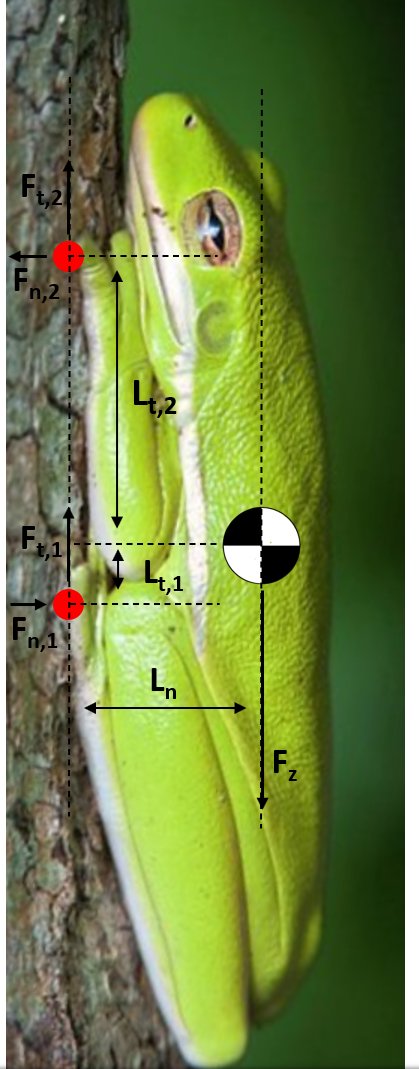
\includegraphics[width=4cm, height=8cm,angle=0]{images/limb spreading/tree_frog_forces_vertical.PNG}
\caption{}
\label{fig:tree_frog_with_forces}
\end{subfigure}
\hspace{0.8in}
\begin{subfigure}{0.24\textwidth}
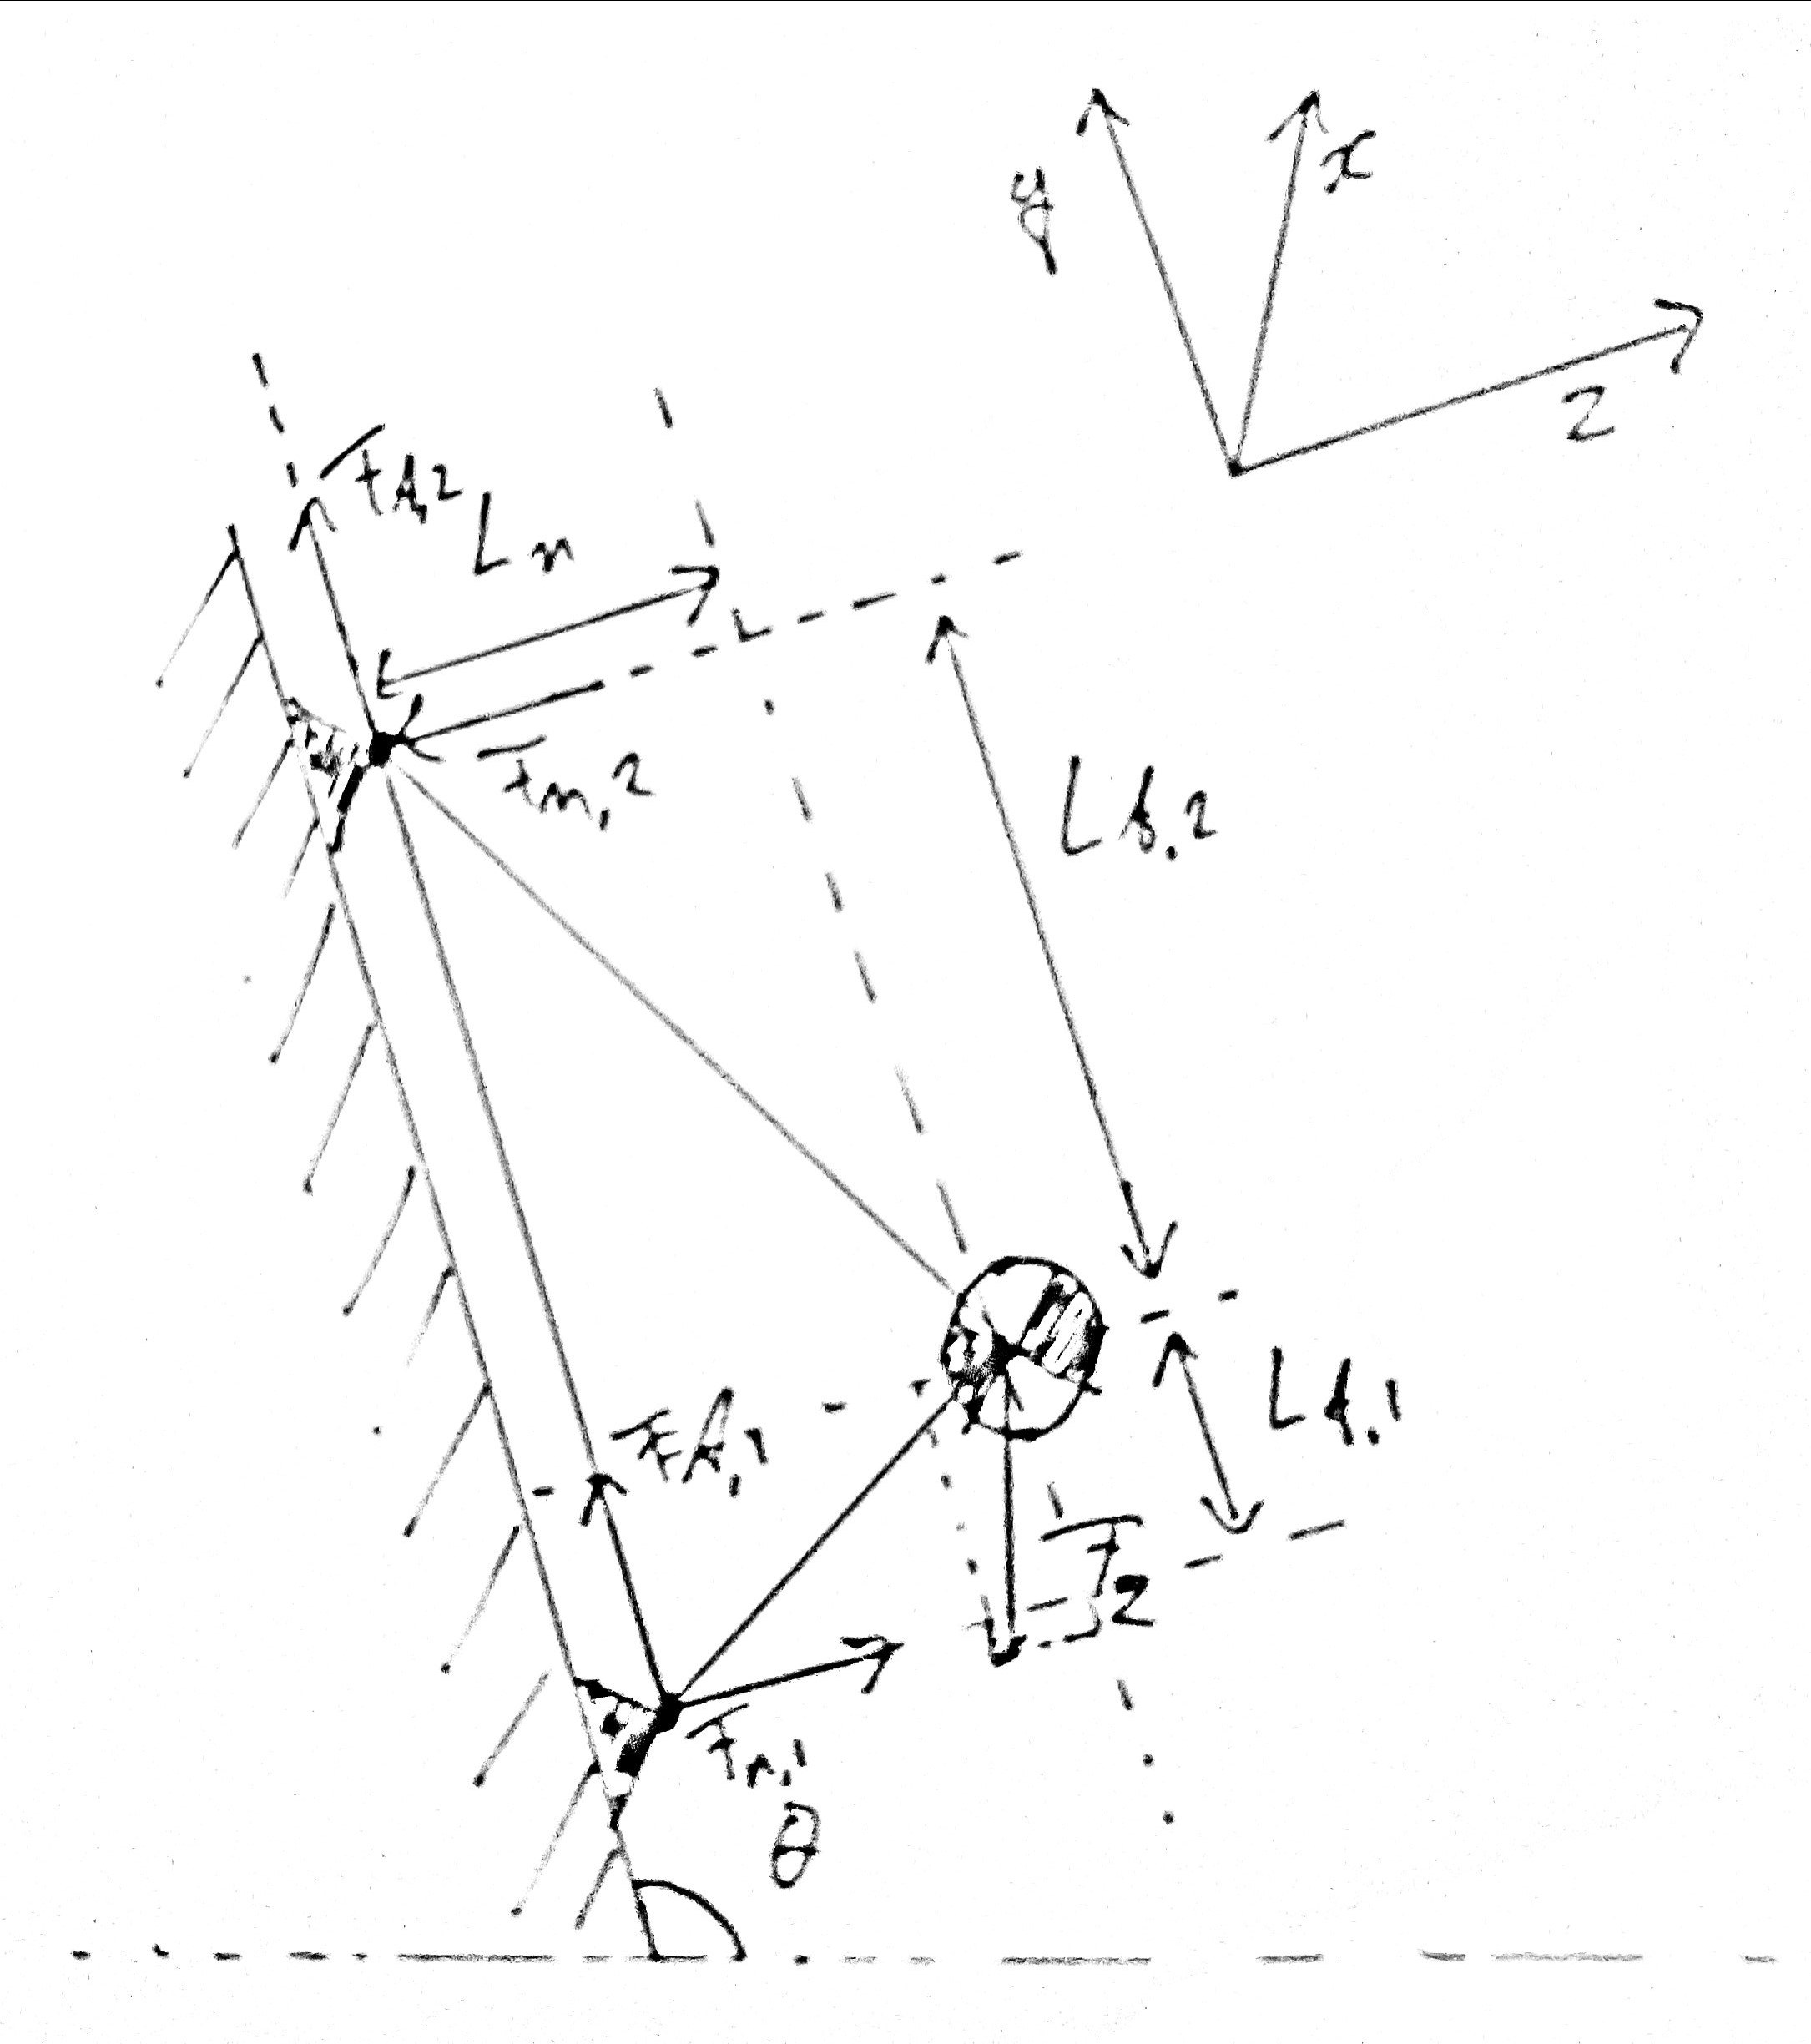
\includegraphics[width=5cm, height=8cm, angle=0]{images/limb spreading/FBD_frog_angle.jpg}
\caption{}
\label{fig:FBD_2D}
\end{subfigure}
\caption{Forces on a tree frog in resting position with in (a) the Hyla Cinerea with the relevant forces and dimensions and in (b) the free body diagram of the same situation}
\label{fig:FBD_tree_frog}
\end{figure}

\qquad The normal forces acting on the limbs of the frog can be fully defined using static equilibrium equations. The tangential forces however, can not be easily determined because the problem is statically over constrained and thus static indeterminate. Typically, such problems can be solved when the mechanical properties of the rigid body are known. The mechanical properties of the body of the tree frog connecting the two attachment points are dependent on the tree frog and can therefore not be easily determined. Furthermore, the tangential forces can be manipulated by the frog itself. The frog can create a force between the limbs with the application of a proximal pull. This proximal pulling is also described in Section \ref{sec:intro_spreading} and is visible in Figure \ref{fig:limb_spreading_rest}-\ref{fig:limb_spreading_second_spread}. The behaviour visible is displayed by the frog when the surface the frog is sitting on, is rotated so that the frog needs a larger adhesional force in order to prevent falling off.\\ 

\qquad The forces at the surface of the adhesive pads are visible in Figure \ref{fig:frog_feet}. The proximal pulling forces $F_{p,1}$ and $F_{p,2}$ are oriented towards the center of gravity and can be decomposed in the x and y-components. 

\begin{figure}[h!]
    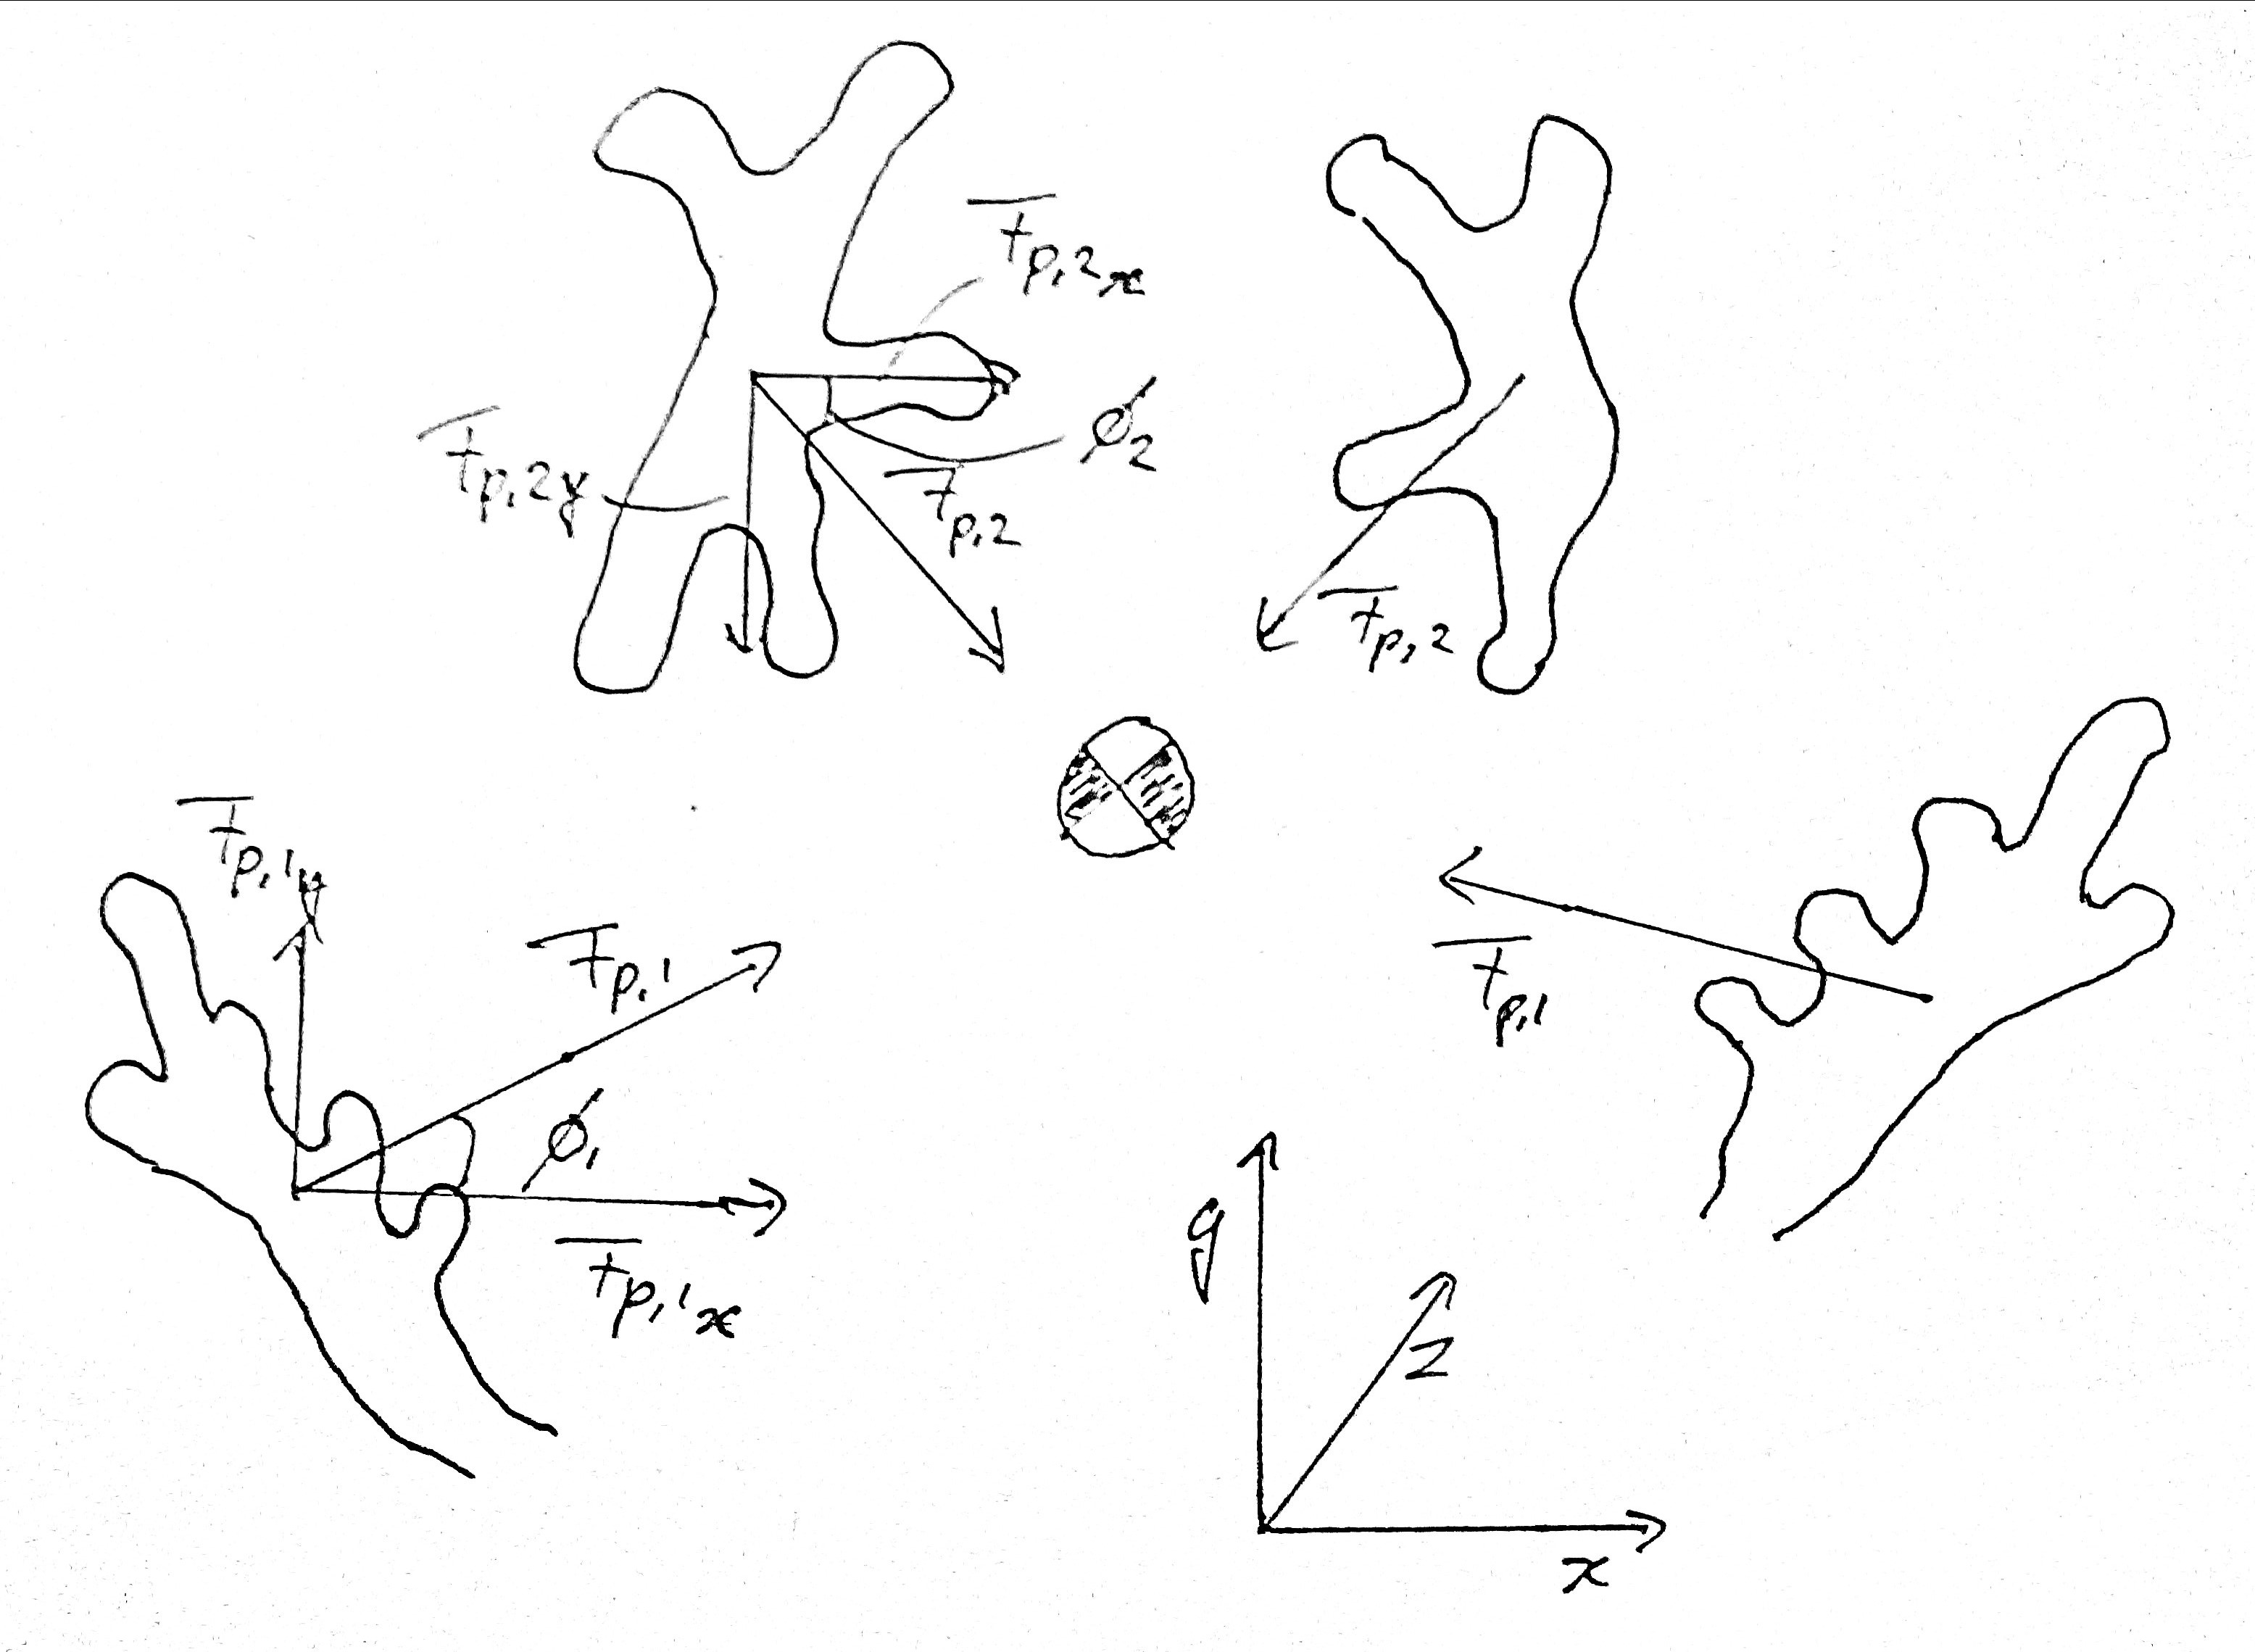
\includegraphics[width=0.65\linewidth, height=7cm, angle=0]{images/limb spreading/frog_feet_streched.jpg}
    \caption{The adhesive surfaces on the frog feet seen from below. The proximal pulling forces $F_{p,1}$ and $F_{p,2}$ are decomposed in force components in the x-direction as $F_{p,1_x}$ and $F_{p,2_x}$. The force components in the y-direction are represented by $F_{p,1_y}$ and $F_{p,2_y}$.}
    \label{fig:frog_feet}
\end{figure}

\qquad The limb spreading does also influence the angles of attachment $\alpha_{1}$ and $\alpha_{2}$ as visible in Figure \ref{fig:frog_schematic}. The tangential forces on the adhesive surfaces of the frog are split up in a component representing the proximal pulling $F_{p}$ and in components representing the rest of the tangential force on the adhesive surfaces, $F_{s,1}$ and $F_{s,2}$. The magnitude of $F_{s,1}$ and $F_{s,2}$ is unknown because the FBD of the frog is statically indeterminate and we do not known the stiffness properties of the frog body connecting the two points of attachment. The relations between these various force components are given by the relations visible in Equation \ref{eq:tangential_forces}.\\ 

\begin{figure}[h!]
    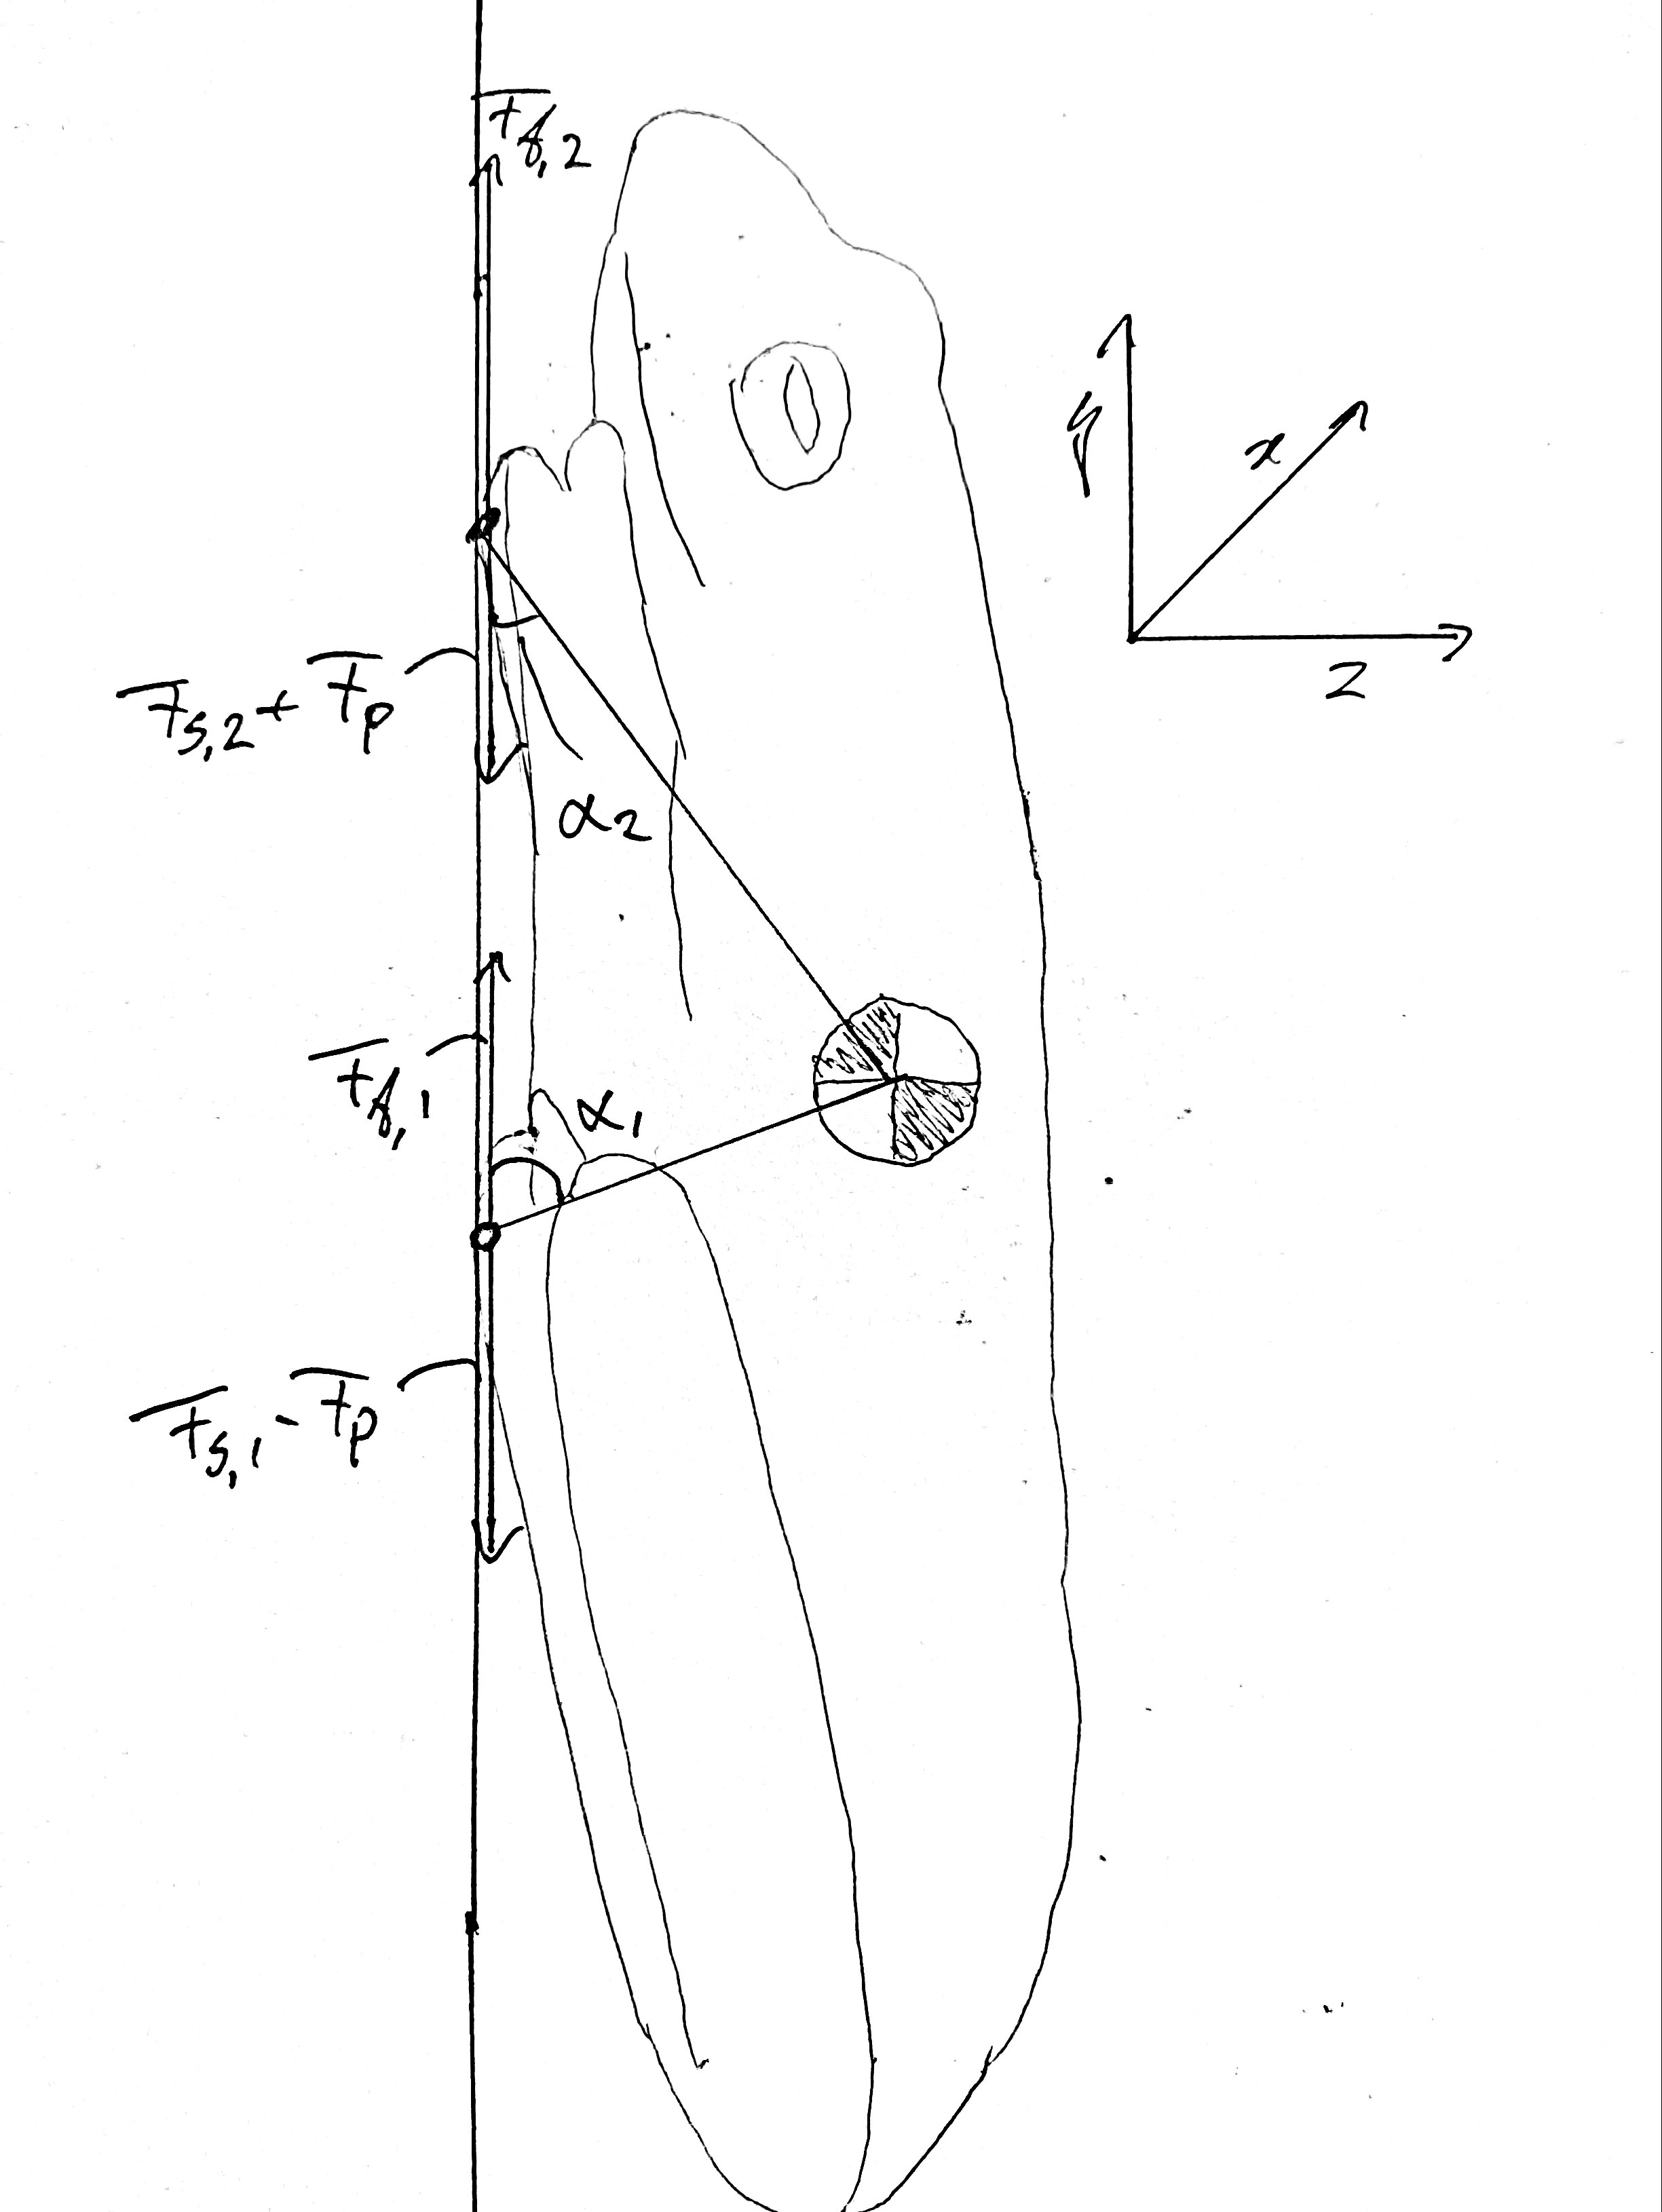
\includegraphics[width=0.55\linewidth, height=7.5cm, angle=0]{images/limb spreading/frog_schematic.jpg}
    \caption{2D side view of the frog adhered to a surface at $\theta = \frac{\pi}{2}$. The angles of attachment are $\alpha_{1}$ and $\alpha_{2} $}
    \label{fig:frog_schematic}
\end{figure}

\begin{gather}
     F_{t,1} = F_{s,1} - F_{p},\nonumber\\[1ex]
     F_{t,2} = F_{s,2} + F_{p},\nonumber\\[1ex]
     F_z = F_{t,1} + F_{t,2}    
     \label{eq:tangential_forces}
\end{gather}

\qquad A Matlab model is written in which three cases are defined. The first case considers a frog that does not make use of proximal pulling. The mechanical properties of the frog body connecting the two points of attachment are assumed as such that the tangential forces are both equal to half of the tangential component of the gravitational force $F_{t,1} = F_{t,2} = \frac{F_{z}}{2} cos(\frac{\pi}{2} - \theta)$. The normal forces are calculated using the relations given in Equation \ref{eq:static_equilibrium_normal}.\\

\begin{gather}
     F_{n,2} = \frac{F_z (L_n cos(\frac{\pi}{2} - \theta) + L_{t,1} cos(\theta))}{L_{t,1} + L_{t,2}},\nonumber\\[1ex]
     F_{n,1} = \frac{F_{z} cos(\frac{\pi}{2} - \theta) L_{n} - L_{t,2} F_{n,2}}{L_{t,1}}
     \label{eq:static_equilibrium_normal}
\end{gather}

\qquad The second case involves a situation in which the frog proximally pulls its limbs. The magnitude of these pulling forces is derived from the work of Endlein et al. \cite{endlein2013sticking} which is also discussed in Section \ref{sec:intro_spreading}. It is assumed that the proximal pulling starts when the frog performs its first spread. The proximal pulling forces increase to their maximal values when the frog performs its second spread. The angles of the first and second spread are taken form the work of Endlein et al. and are $ \theta_1 = 106 [deg]$ and $\theta_2 = 131 [deg]$ respectively. Equations \ref{eq:spreading_forces_0} - \ref{eq:spreading_forces_2} give the magnitudes of the pulling forces as a function of parameter $R$ which resembles the ratio of the body weight of the frog and the magnitude of the pulling force. The value of this parameter is $R = 0.2$ as discussed in Section \ref{sec:intro_spreading}. The parameter $\phi_1$ is the angle of the proximal pulling force as visible in Figure \ref{fig:frog_feet}. 

\begin{gather}
     \text{For } \theta > \theta_{1},\nonumber\\[1ex]
     F_{p,1_x} = F_{p,2_x} = F_{p,1_y} = F_{p,2_y} = 0
     \label{eq:spreading_forces_0}
\end{gather}

\begin{gather}
     \text{For } \theta_{1} \leq \theta \geq \theta_2,\nonumber\\[1ex]
     F_{p,1_x} = F_{p,1_x} = F_z \frac{R}{4},\nonumber\\[1ex]
     F_{p,1_y} = tan(\phi_1)  F_{p,1_x} \quad \text{\&} \quad F_{p,2_y} = tan(\phi_1)  F_{p,2_x}
     \label{eq:spreading_forces_1}
\end{gather}

\begin{gather}
     \text{For } \theta > \theta_2,\nonumber\\[1ex]
     F_{p,1_x} = F_{p,1_x} = F_z R,\nonumber\\[1ex]
     F_{p,1_y} = tan(\phi_1)  F_{p,1_x} \quad \text{\&} \quad F_{p,2_y} = tan(\phi_1)  F_{p,2_x}
     \label{eq:spreading_forces_2}
\end{gather}

\qquad The third cases includes the pulling forces as in case 2 but also includes a positional adjustment of the frog due to the re positioning of the limbs. For $\theta_{1} \leq \theta \geq \theta_2$ the dimensions $L_{t1}\ \&\ L_{t2}$ are multiplied with a factor $\frac{3}{2}$ and parameter $L_{n}$ is multiplied with a factor $\frac{3}{4}$. For the second spread the parameters are multiplied with factors $2$ and $\frac{1}{2}$ for $L_{t1}\ \&\  L_{t2}$ and $L_{n}$ respectively. These values are based on a rough estimate derived from images of the tree frog during its different spreading positions as visible in Figure \ref{fig:tree_frog_limb_spreading}.\\


\qquad The forces involved  for the three cases considered are visible in Figures \ref{fig:case_1}, \ref{fig:case_2} and \ref{fig:case_3}. The normal forces are the same for case 1 and 2 since they are independent of the tangential forces. The tangential forces which are dependent on the proximal pulling are different between case 1 and 2. The value of the tangential components $F_{t,1}$ and $F_{t,2}$ increases with the first spread and with the second spread. The increase of the tangential force components after the first spread is relatively small compared to the increase at the second spread which is proportional to the magnitude of the proximal forces visible in Figure \ref{fig:pulling}. Case 3 shows the forces at the contact interface for a combination of proximal pulling and positional adjustment. It is visible that the tangential components increase as also visible for case 2. The normal force components decrease due to the positional adjustment.\\


\begin{figure}[h!]
    \begin{subfigure}{0.48\textwidth}
    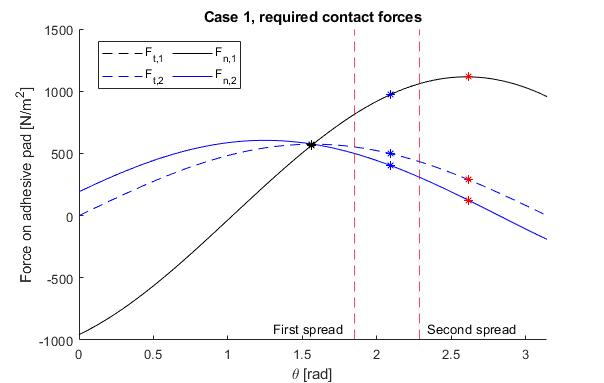
\includegraphics[width=\textwidth, height=5cm, angle=0]{images/limb spreading/FBD_case_1.jpg}
    \caption{}
    \label{fig:case_1}
    \end{subfigure}
    \hfill
    \begin{subfigure}{0.48\textwidth}
    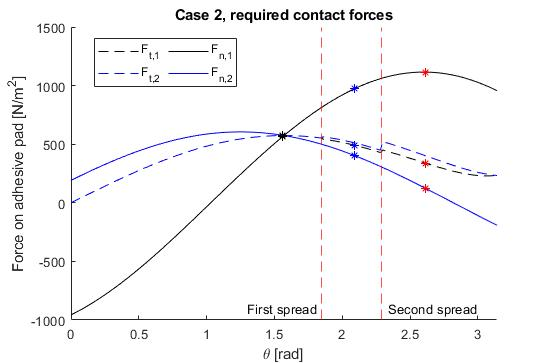
\includegraphics[width=\textwidth, height=5cm, angle=0]{images/limb spreading/FBD_case_2.jpg}
    \caption{}
    \label{fig:case_2}
    \end{subfigure}
    \hfill
    \begin{subfigure}{0.48\textwidth}
    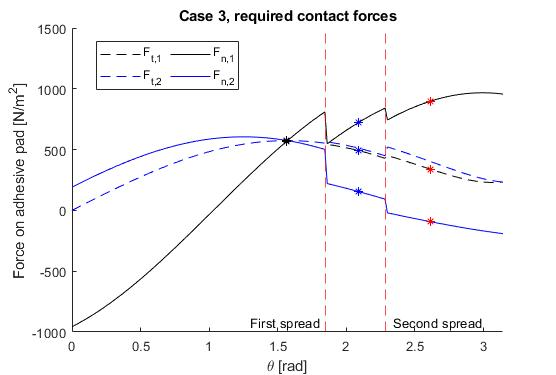
\includegraphics[width=\textwidth, height=5cm, angle=0]{images/limb spreading/FBD_case_3.jpg}
    \caption{}
    \label{fig:case_3}
    \end{subfigure}  
    \begin{subfigure}{0.48\textwidth}
    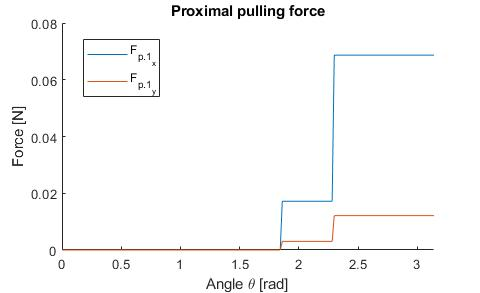
\includegraphics[width=\textwidth, height=5cm, angle=0]{images/limb spreading/pulling_force.jpg}
    \caption{}
    \label{fig:pulling}
    \end{subfigure} 
    \caption{Required contact forces as a function of the the angle $\theta$ for the three cases. The first case in (a) has zero value for every value of $\theta$. In (b), the proximal pulling is included and in (c) positional adjustment is added. The proximal pulling forces for cases 2 and 3 are visible in (d).}
    \label{fig:proximal_pulling_cases}
\end{figure}



\subsection{Discrete fiber model}
\subsubsection{Model fundamentals}\label{sec:discrete_model_fundamentals}
The aim of the discrete fiber model is to replicate the mechanical properties of the epithelial layer by closely mimicking the epithelial geometry and the properties of the various components of the epithelial cell as visible in Figure \ref{fig:epithelial_cell_components}. 


\subsubsection{Model implementation: Geometry}\label{sec:discrete_model_geometry}
The outline of the epithelial cell and its cell components can be seen in Figure \ref{fig:epithelial_cell_components}. The basic outline of the cell and the keratinous part in the the cell are implemented in a 2D model. This model uses  a parameterized Matlab model in which the fibres are proportionally divided over the keratinous domain containing the fibers. This 2D model can be implemented in Solidworks and from Solidworks it can be transferred into Comsol Multiphysics. The Solidworks implementation is visible in Figure \ref{fig:geometry_solidworks}.\\ 

\begin{figure}[h!] 
     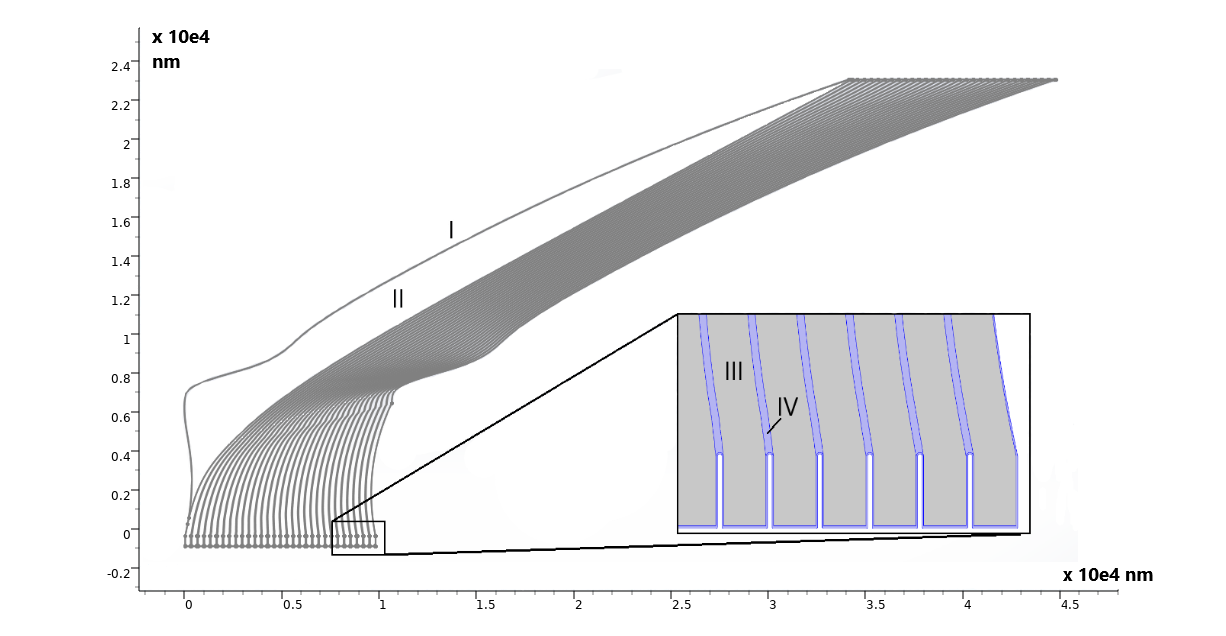
\includegraphics[width=0.85\linewidth, height=6.5cm, angle=0]{images/discrete_model_implementation/solidworks geometry_schematic.png}
     \caption{A representation of the geometry implemented in Solidworks. The keratinous structure is visible in the right part of the cell. The enlarged section shows the individual keratinous fibres. $I$ represents the cornified cell envelope, $II$ the lymph space, $III$ a keratinous fibre and $IV$ the space between the keratinous fibres with forms the matrix in which the fibres are embedded.}
     \label{fig:geometry_solidworks}
\end{figure}

\qquad The geometry visible in Figure \ref{fig:geometry_solidworks} has a relatively high level of complexity due to the presence of the discrete fibers. Comsol Multiphysics needs a mesh in order to perform the finite element analyses. The amount of elements of this mesh increases with the complexity of the geometry and the high level of complexity of the geometry visible in Figure \ref{fig:geometry_solidworks} causes the mesh builder to form a mesh that contains a very large number of mesh elements as visible in Figure \ref{fig:mesh}. The number of mesh elements directly influences the convergence speed of the model. The fiber configuration visible in Figure \ref{fig:geometry_solidworks} however, can be significantly simplified into a rectangular geometry with a reduced number of fibers. The implications of this simplifications are discussed in Section \ref{sec:}.\\

\begin{figure}[h!] 
    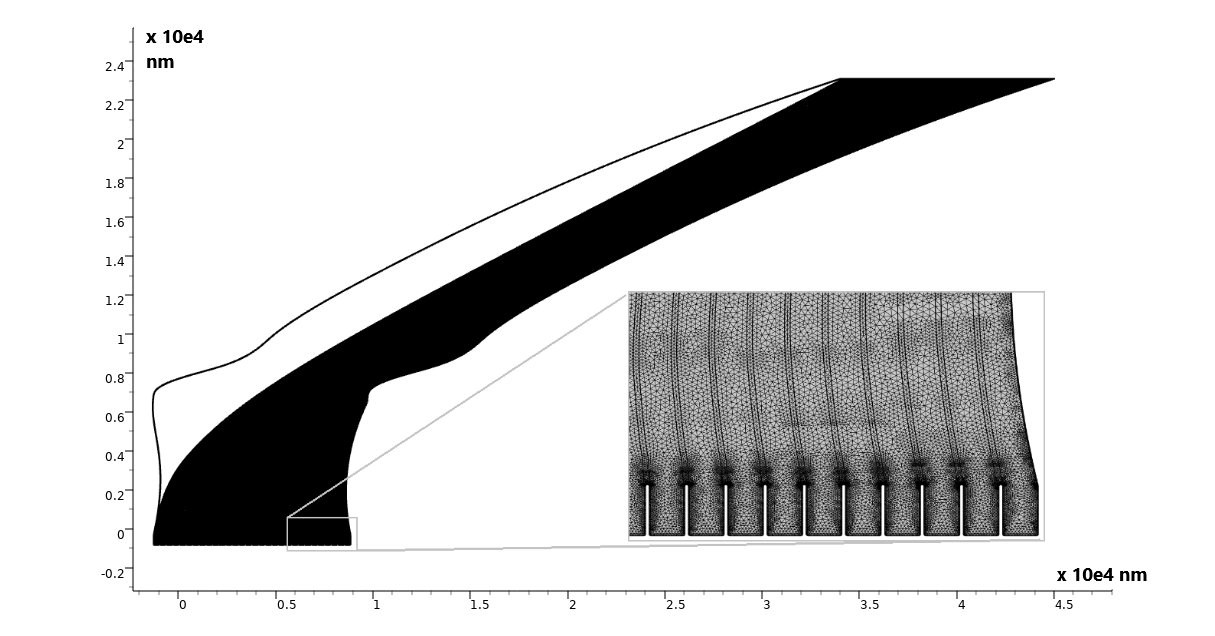
\includegraphics[width=0.85\linewidth, height=6.5cm, angle=0]{images/discrete_model_implementation/mesh_compleet.png}
    \caption{The very dense mesh for the geometry in which one fibre bundle runs from every pillar. This mesh consists of 715790 domain elements and 118113 boundary elements.}
    \label{fig:mesh}
\end{figure}

\qquad The fiber density and the amount of fibers is varied between models to evaluate the consequences of these changes. The standard size of an simplified square fibrous domain is $10\mu m$ in width and $20 \mu m$ in height. This size has the order of magnitude as the size of an epithelial cell. The pillars of the epithelial cell are described to play a role in the establishment of contact between the epithelial layer and the substrate while the channels between the pillars drain excess fluids from the adhesive pads \cite{kappl2016nanoscale}. The pillars however are not described to play a role in the stress distribution along the pad when contact is established and are therefore neglected in the simplified model.


\subsubsection{Model implementation: boundary conditions}\label{sec:discrete_model_boundary_con}
The boundary conditions used in the model resemble the mechanical properties of the epithelial cell layer of the tree frog and need to such that the model is loaded in a similar way as an epithelial cell.\\ 

\begin{figure}[h!] 
    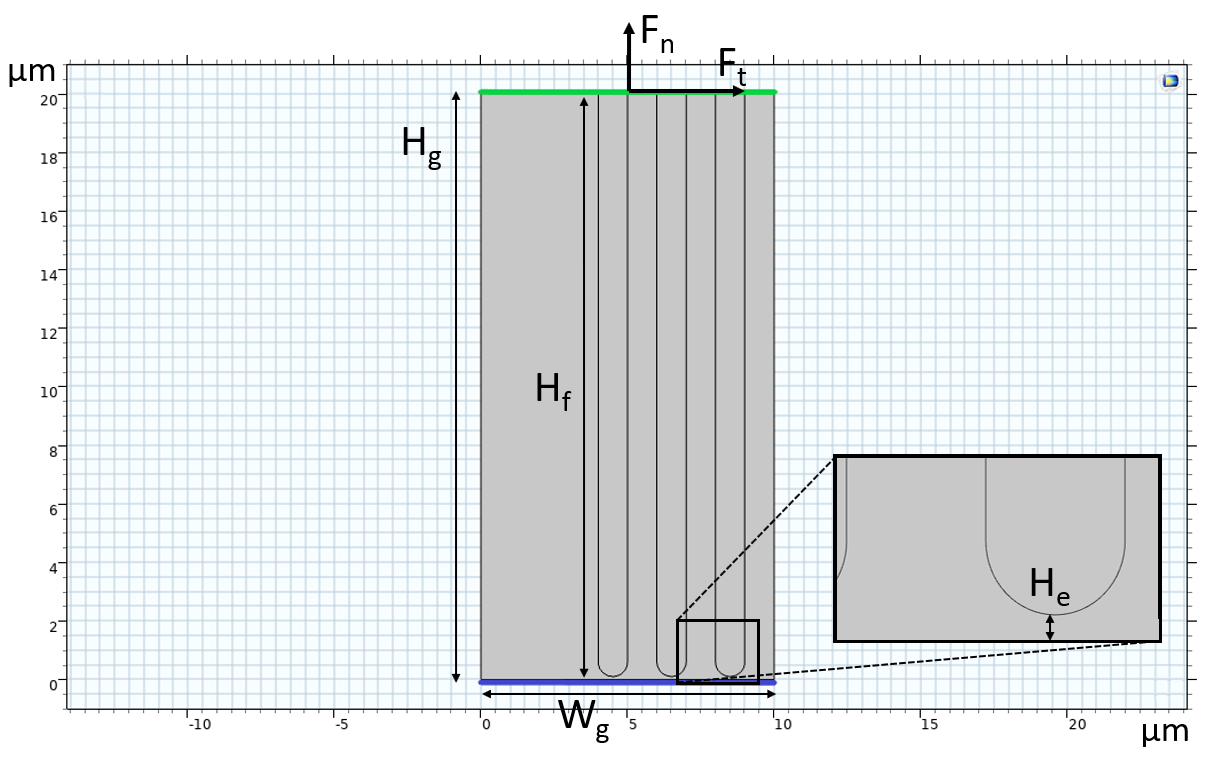
\includegraphics[width=0.8\linewidth, height=7.5cm, angle=0]{images/discrete_model_implementation/lever_distance.png}
    \caption{The dimensions involved in the boundary conditions of the simplified domain. The upper boundary is coloured green and is the point of application for the applied forces $F_n \& F_t$. The lower boundary is colored blue. The height and width of the domain are represented by $H_g \& W_s$ respectively. $H_f$ represent the length of the fibers and $H_e$ represent the distance between the fiber tips and the lower boundary.}
    \label{fig:boundary_conditions}
\end{figure}

\qquad The points of attention that to be addressed to obtain the required mechanical response for the simplified model with the rectangular domain are:
\begin{enumerate}
    \item The lower boundary of the domain is assumed fixed. This boundary condition can be applied since the contact with the substrate is assumed to be constant. The constant contact with the substrate also allows stress concentrations on the substrate do develop. This makes the mechanical behaviour more pronounced compared to a situation in which the lower boundary can adjust to applied loads. The geometry edges to which the boundary conditions are applied are visible in Figure \ref{fig:boundary_conditions}.
    \item Forces are applied on the upper boundary. This configuration resembles a situation in which the tree frog exerts a force on the substrate. This loading configuration is a simplification of the real situation in which the load would be more distributed over the domain. This is not considered an issue for a normal load $F_n$ since the flow direction of the stresses in the material is orthogonal to the upper boundary used for the load application in the simulation. A shear load $F_t$ however, induces a moment in the material which is dependent on the distance $H_g$ between the lower boundary and the plane of force application. This moment is less when the force is applied over the whole domain which shortens the length of the lever to $\frac{H_g}{2}$.
    \item The upper boundary is free in translation in the x and the y-direction but constrained in rotation. The rotational constraint is derived from the observation that the epithelial cells are concatenated and would therefore resist rotation of the upper boundaries. Fully constrained rotation is a simplified assumption of the real situation since the real situation would most probably offer a small amount of rotational freedom.
    \item The left and right sides of the geometry are left free. Although an epithelial cell is in constant contact with its surrounding cells on the sides, it can be assumed that all these cells are loaded in a similar way. This would result in a similar deformation pattern for neighbouring cells and with that no significant additional loads on the right and left boundaries of a simplified rectangular domain. 
    \item In Section \ref{sec:bio_material_properties} the stiffness of the individual epithelial cell components is discussed. These stiffness values are also used in the discrete fiber model. The influence of the variation of the stiffness for the different components is discussed in Section \ref{ch:results}.
    \item The simplified model uses a linear elastic material model for the fibers and the base material. This assumption is made after an evaluation of the differences between a hyperelastic and a linear elastic material model. The sensitivity of the simplified model is further evaluated in Section \ref{sec:discrete_model_sensitivities}.
    \item The length of the fibers $H_f$ and the size of the gap $H_e$ between the fiber tips and the substrate are kept constant for all the performed simulations. The thin layer ensures that the contact with the substrate is established with a continuous domain. This is a simplification of the real situation in which the contact is established with the thin cornified cell envelope which is also made visible in Figure \ref{fig:epithelial_cell_components}.
    \item The bonding between the fibers and the base material is assumed perfect in the simplified model which means that the stiffness of the bonding is equal to the stiffness of the most compliant material involved. The influence of this assumption and the impact of a change in the bonding between fibers and matrix is discussed in Sections \ref{sec:results_fiber_bonding} and \ref{sec:discrete_model_sensitivities}.
\end{enumerate}



\subsubsection{Model validation}\label{sec:discrete_model_validation}
Validation of the discrete fiber model is done by comparing the results of the discrete fiber model with the results obtained by Xue et al. \cite{xue2017hybrid}. These results are described in Section \ref{sec:tree_frog_applications}.\\

\qquad When a rectangular block of material uniform elastic or hyperelastic properties with a fixed base is loaded in tension, the stress concentrations are found at the corners of the geometry as is visible in Figure \ref{fig:uniform_elastic_stress}. The S22 stress component considered is equivalent to the S33 stress component considered by Xue et al. as visible in Figure \ref{fig:Xue_model_1} and \ref{fig:Xue_model_2}. The stiffness of the homogeneous material is set to $2 MPa$ with a Poison's ratio of $0.49$.\\

\begin{figure}[h!]
    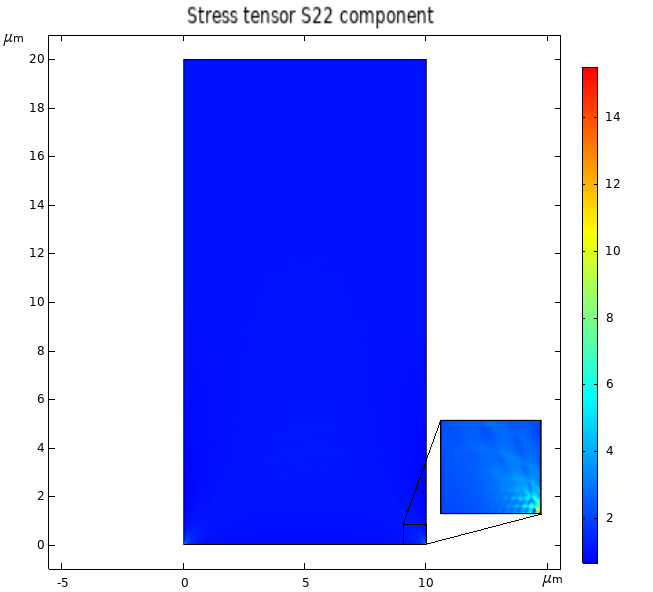
\includegraphics[width=0.7\linewidth, height=8.5cm, angle=0]{images/discrete_model_validation/blok_elastic.png}
    \caption{An uniform elastic domain with a fixed base loaded with a vertical load on the upper domain. The stress concentrations appear in the lower right and left corners. The stress concentration in the lower right corner is visible in the insert. The S22 component of the stress is considered.}
    \label{fig:uniform_elastic_stress}
\end{figure}

\qquad The stress distribution in the uniform domain can be compared with the stress distribution in a domain in which fibers are implemented. Figure \ref{fig:coarse_fibers} shows a domain in which coarse fibers are implemented. The stress is strongly influenced by the location of the fiber re-enforcement. The most important observation is that the fibre re-enforced model has a much lower value for the stress at the end of the geometry at $L = 10 \mu m$ on the horizontal axis. This reduction in peak stress increases the adhesive strength of the material since the stress are better divided over the contact interface compared to the uniform domain visible in Figure \ref{fig:uniform_elastic_stress}. The stiffness of the base material used for this model is $2 [MPa]$ and the stiffness of the fibers is set to $200 [MPa]$. A Poison's ratio of $0.49$ is implemented for the base material and the fibers.\\

\begin{figure}[h!]
    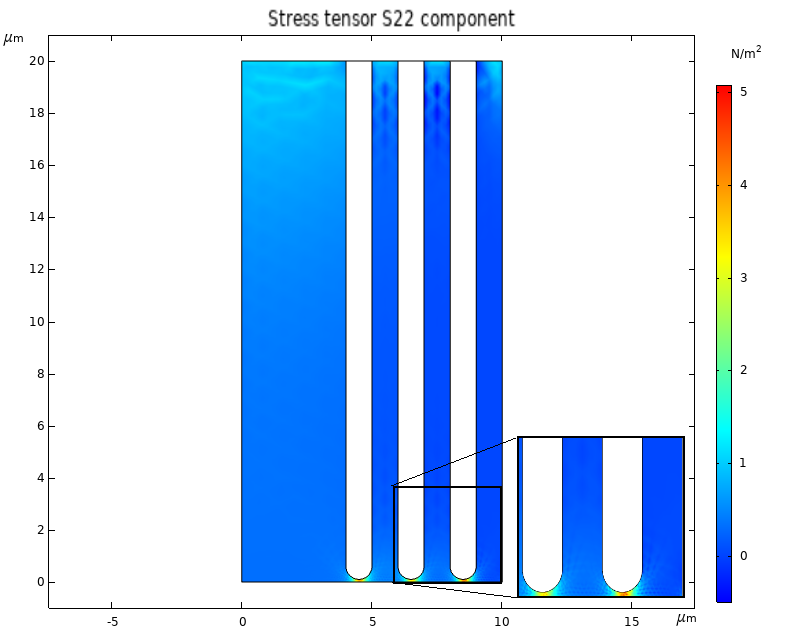
\includegraphics[width=0.7\linewidth, height=8.5cm, angle=0]{images/discrete_model_validation/coarse_fibers.png}
    \caption{A composite model with coarse fibers implemented in a relatively soft base material. The loading and boundary conditions of this model are similar to the model from Figure \ref{fig:uniform_elastic_stress}.}
    \label{fig:coarse_fibers}
\end{figure}

\qquad The stress concentrations visible in Figure \ref{fig:coarse_fibers} are very similar to what is visible in Figure \ref{fig:Xue_model_1}. In both models, a stress concentration occurs between the fibers and the contact surface. When the maximum of the stress magnitude is compared between Figure \ref{fig:uniform_elastic_stress} and Figure \ref{fig:coarse_fibers} it appears that the magnitude of the stress below the fibers in Figure \ref{fig:coarse_fibers} is significantly lower than the magnitude of the stress in the lower right corner of the geometry as visible in Figure \ref{fig:uniform_elastic_stress}. The maximum of the stress found in the composite material is a factor $\frac{15}{5} = 3$ lower than the maximum value of the stress in the continuous material domain.\\ 

\qquad These observations confirm that the stresses in the simplified composite model are indeed lower than the stresses in a geometry with homogeneous material properties. Furthermore, it is observed that the location of the maximum stress shifts from the corner of the geometry to a location under the fibers. These observations are also described by Xue et al. and validate the use of the simplified composite model.


\subsubsection{Model sensitivities}\label{sec:discrete_model_sensitivities}
This section describes the sensitivity of the discrete model to numerical effects and solver configurations. The sensitivity of the discrete fiber model to variation in model variables is described in Section \ref{sec:results_fiber_stiffness} and \ref{sec:results_fiber_bonding}.\\


% een sensitivity analysis generally describes the influence of a change in one of the model variables. The variables relevant for such a study in the case of the discrete model are:
%    - stiffness of the layer between the fibers and the base material
%    - Material model used for the base material
%    - Numerical instability due to the mesh density

% hier beschrijven

% hier ook de gevoeligheid voor ruis en meenemen, dit komt dan vervolgens weer terug in het gedeelte van de data processing

%  The adaptive mesh refinement algorithm will globally adjust the mesh to better resolve the local stresses, and these stresses depend on the solution everywhere else in the model. The solution smoothens out but takes to much mesh elements for the amount of memory available to fully smoothen out.(this partly works but is not the best option to come to a smooth solution)
%     https://www.comsol.com/blogs/using-adaptive-meshing-local-solution-improvement/
%     - smoothing is always an option...and is also done in the post-processing


\qquad The stress response of the model influenced numerical instability that is related to the mesh density and also known as the Runge's phenomenon. This phenomenon causes oscillation at the edges of an interval when a polynominal interpolation is used. This phenomenon can be countered by increasing the resolution of the mesh. This method increases the amount of mesh nodes. A more efficient way is a mesh refinement study that increases the mesh locally at the locations where steep gradients are encountered. The adaptive mesh algorithm does smooth the response but takes too much mesh elements for the available memory to compute a fully smooth model response.\\

\qquad Another way to smooth the response is an increase in the discretization order of the displacement field. Increasing the discretization order also increases the memory needed for the computation and causes memory errors when the discretization order is too large. An increase in the discretization order however, significantly smooths out the solution as is visible in Figure \ref{fig:discretization_order}.\\

\begin{figure}[h!]
    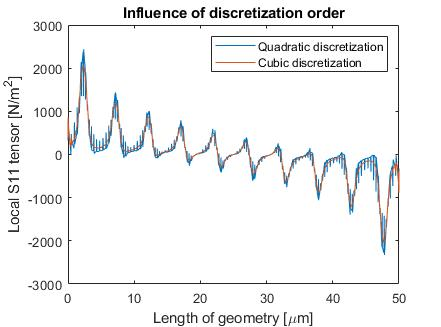
\includegraphics[width=0.65\linewidth, height=7cm, angle=0]{images/discrete_model_sensitivities/Influence_discretization_order.jpg}
    \caption{Model stress response for different discretization orders. The cubic discretization gives a smoother response than the quadratic discretization but is more computational demanding.}
    \label{fig:discretization_order}
\end{figure}

\qquad The discrete fiber model that uses linear elastic material properties does encounter non-linear behaviour is certain loading configurations. This is the case when a shear and a normal load are simultaneously applied. This non-linear behaviour can lead to convergence issues. To prevent these and to shorten computation time the estimates of the initial values of the dependent values need to be chosen carefully. Comsol Multiphysics uses these values as an estimate for the computational result and therefore benefits from an accurate prediction of these values.\\ 
    
    

\subsubsection{Data processing}\label{sec:discrete_model_data}
% hier beschrijven hoe je de data uit het comsol model heb gekregen en hoe je deze data daarna verwerkt hebt in Matlab. Dit kan allemaal kort en bondig!

The stresses of the discrete fiber model are evaluated at the lower boundary of the geometry. The values of the stress components are evaluated in a cut line which is defined just above the lower geometry boundary at $y = 0.001 \mu m$. The $S_{11}$ and $S_{22}$ stress components are extracted from the Comsol simulation.\\ 

\qquad The discretization order of the displacement field in the Comsol model is set to quadratic. In Section, it was discussed that this discretization can be increased to produce a smoother stress response. This however significantly increases the computational demands of the model. The discretization order of the model is therefore not increased and the results are smoothed out using a moving average in the post-processing of the results. This produces similar results compared to the results that are produced with a higher discretization order.\\


\subsection{HGO model}\label{sec:HGO_model}
The HGO model allows the implementation of of directional dependent properties in a model. This allows the implementation composite material properties in a continuous domain. This reduces the amount of mess elements needed for the implementation of composite material properties.

\subsubsection{Model fundamentals}\label{sec:HGO_model_fundamentals}
The formulation of the possible linear material transformations for an orthotropic material is visible in Equation \ref{eq:general_transformation} which shows the stress vector $\sigma$, the strain vector $\epsilon$ and the fourth order stiffness tensor $C$ \cite{freutel2014finite}. The material properties of an orthotropic material are different along the orthogonal axis of the material.\\ 

\begin{gather}
    \sigma = C \epsilon,\nonumber\\[1ex]
    \text{With for $\sigma$, $\epsilon$ and $C$:}\nonumber\\[1ex]
    \sigma  = \begin{bmatrix}
    \sigma_{11}\\
    \sigma_{22}\\
    \sigma_{33}\\
    \sigma_{23}\\
    \sigma_{13}\\
    \sigma_{12} \end{bmatrix},\quad
    \epsilon = \begin{bmatrix}
    \epsilon_{11}\\
    \epsilon_{22}\\
    \epsilon_{33}\\
    2 \epsilon_{23}\\
    2 \epsilon_{13}\\
    2 \epsilon_{12} \end{bmatrix},\nonumber\\
    C = \begin{bmatrix}
    C_{1111} & C_{1122} & C_{1133} & 0 & 0 & 0\\
    C_{2211} & C_{2222} & C_{2233} & 0 & 0 & 0\\
    C_{3311} & C_{3322} & C_{3333} & 0 & 0 & 0\\
    0 & 0 & 0 & C_{2323} & 0 & 0 \\
    0 & 0 & 0 & 0 & C_{1313} & 0 \\
    0 & 0 & 0 & 0 & 0 & C_{1212} \end{bmatrix},\nonumber\\[1ex]
    \text{With}\nonumber\\[1ex]
    C_{2211} = C_{1122}, C_{3311} = C_{1133}, C_{3322} = C_{2233}
    \label{eq:general_transformation}
\end{gather}

\qquad Biological materials often have similar properties in two orthogonal directions. This is caused by the (local) orientation of the fibers in these biological materials. The modifications needed to represent such a transversal isotropic material by the fourth order stiffness tensor $C$ from Equation \ref{eq:general_transformation} are visible in Equation \ref{eq:mod_stiffness_tensor} \cite{freutel2014finite}.

\begin{gather}
    C_{2211} = C_{1122}, C_{3311} = C_{1133} = C_{3322} = C_{2233},\nonumber\\
    C_{1111} = C_{2222},\nonumber\\
    C_{2323} = C_{1313},\nonumber\\
    C_{1212} = \frac{1}{2}(C_{1111} - C_{1122})
    \label{eq:mod_stiffness_tensor}
\end{gather}

\qquad These equations allow the implementation of direction-dependent material properties but represent only linear material deformations. The fibres in biological materials however, often display non-linear material behaviour. Fibres are often much stiffer in tension than in compression \cite{li2009three} and can also display strain-dependent elastic properties. Hyperelastic material properties can be described with several material models. Examples of such models are the neo-Hookean material model \cite{ogden1997non} and the Mooney–Rivlin model \cite{mooney1940theory}.\\

\qquad In order to model the non-linear properties of the materials present in the epithelial cell of the tree frog, a material model is needed that describes material behaviour of the fibers and the ground substance in which the fibres are embedded. The fiber orientation in the keratinous domain of the epithelial cell is a function of the location which makes the material properties direction and location dependent.\\

\qquad The HGO model introduced by Holzapfel et al.\cite{holzapfel2000new} can be used to implement the directional and location dependent material behaviour. This model allows modelling of composite fibrous materials with anisotropic hyperelastic properties. These hyperelastic properties can be implemented for both the ground substance and for the embedded fibers. The equations for the HGO model describe the isochoric strain energy density which is defined as visible in Equation \ref{eq:isochoric_strain_energy}. The parameter $W_{1}$ describes the contribution of the material in which the fibres are embedded and $W_{4}$ describes the contribution of the fibres. Both parameters are derived using Equation \ref{eq:F} - \ref{eq:elastic_cauchy_green_tensor}. 
  
\begin{equation}
      W_s = W_{1} + W_{4}
      \label{eq:isochoric_strain_energy}
\end{equation}

\qquad In order to construct the parameters $W_1$ and $W_4$, it is required to go back to some basic relations. The deformation of a material can be described with the deformation gradient $\textbf{F}$ given in Equation \ref{eq:F}. This gradient is composed of a parameter describing the rotation $\textbf{R}$ and of a parameter which describes the translation from the undeformed to the deformed composition $\textbf{V}$. The left Cauchy-Green deformation tensor $\textbf{B}$ can be constructed from the deformation gradient $\textbf{F}$ and is visible in Equation \ref{eq:B}. These basic equations can be used to construct the invariant $\overline{\textbf{I}}_{1}$ which is used to describe the incompressible material behaviour as visible in Equation \ref{eq:invariant_incompressible_mat}. This invariant uses the jacobian $\textbf{J}$ of $\textbf{F}$ and the invariant $\textbf{I}_{1}$ with is defined as $\textbf{I}_{1} = tr(\textbf{B})$.

\begin{equation}
    \textbf{F} = \textbf{V} \textbf{R} 
    \label{eq:F}
\end{equation}

\begin{equation}
    \textbf{B} = \textbf{F} \textbf{F}^T = \textbf{V}^2
    \label{eq:B}
\end{equation}

\begin{equation}
    \overline{\textbf{I}}_{1} = \textbf{J}^{- \frac{2}{3}} \textbf{I}_{1}
    \label{eq:invariant_incompressible_mat}
\end{equation}

\qquad The invariant $\textbf{I}_4$ is dependent on the direction of the fibres and on the local deformation gradient. Equations \ref{eq:I4_short} and \ref{eq:I4_long} show the short and the long notation of the invariant respectively. The invariant is composed of a vector field $\textbf{a}$ which represents the direction of the fibres and the isochoric elastic Cauchy-Green tensor $\overline{C_{el}}$.

\begin{equation}
    I_{4} = \textbf{a} \overline{\textbf{C}_{el}} \textbf{a}
    \label{eq:I4_short}
\end{equation}
  
\begin{equation}\label{eq:I4_long}
  \begin{split}
       I_{4} & = a_{1} \overline{C_{el_{11}}} a_{1} 
            + 2a_{1} \overline{C_{el_{12}}} a_{2}
            + 2 a_{1} \overline{C_{el_{13}}} a_{3}\\
            & + a_{2} \overline{C_{el_{22}}} a_{2}
            + 2 a_{2} \overline{C_{el_{23}}} a_{3}
            + a_{3} \overline{C_{el_{33}}} a_{3}
        \end{split}
 \end{equation}
 
 \qquad The isochoric elastic Cauchy-Green tensor $\overline{\textbf{C}_{el}}$ as visible in Equation \ref{eq:elastic_cauchy_green_tensor} is constructed from the local elastic Cauchy-Green tensor $\textbf{C}_{el_{ij}}$ and from the elastic volume ratio $\textbf{J}_{el}$. Subscripts $i$ and $j$ express the local coordinates. $\textbf{C}_{el_{ij}}$ is constructed from the inverse of the inelastic deformation gradient and from the local Cauchy-Green tensor. This local Cauchy-Green tensor is constructed from the local deformation gradients as visible in Equation \ref{eq:local_cauchy-green_tensor}. This equation sums over $n$ dimensions and uses the deformations in the $i$ and in the $j$ directions.

\begin{equation}
    C_{l_{ij}} = \sum_{n=1}^{3} F_{ni} F_{nj}
    \label{eq:local_cauchy-green_tensor}
\end{equation}

\begin{equation}
    \overline{\textbf{C}_{el}}_{_{ij}} = \textbf{J}^{-\frac{2}{3}}_{el} \textbf{C}_{el_{ij}}
    \label{eq:elastic_cauchy_green_tensor}
\end{equation}
  
 \qquad The parameters $\overline{I}_{1}$ and $I_{4}$ can now be used to define the parameters from Equation \ref{eq:isochoric_strain_energy}. $W_1$ is the isotropic function with describes the isotropic behaviour of the material in which the fibres are embedded. This function depends on one material parameter $C_{10}$ and the first invariant of isochoric elastic right Cauchy-Green tensor $\overline{I}_{1}$ as visible in Equation \ref{eq:first_isochoric invariant}. The parameter $W_4$ represents the contribution of the anisotropic material properties. As visible in Equation \ref{eq:anisotropic_w4}, $W_4$ is dependent on the parameters $k_1$ and $k_2$ which respectively represent a stress like material parameter and a dimensionless constant. The invariant $I_4$ is  visible in Equation \ref{eq:I4_long}. The parameter $k_{2}$ represents the amount of non-linearity in the material. This parameter gives the amount of strain stiffening.
  
 \begin{equation}
      W_1 = \frac{C_{10}}{2}(\overline{I_{1}}) - 3)
      \label{eq:first_isochoric invariant}
 \end{equation}
  
\begin{equation}
    W_4 = \frac{k_1}{2k_2}(e^{k_2(I_4 - 1)^2} - 1)
    \label{eq:anisotropic_w4}
\end{equation}

\subsubsection{Model implementation: geometry}\label{sec:HGO_model_geometry}
The working principle of the keratinous structure, is not expected to be dependent on an exact number of fibres. The most important characteristic of the fibrous structure is that of an anisotropic material. Furthermore, it is expected to display non-linear material behaviour. The HGO material model (see section about modelling methods) allows the implementation of anisotropic hyperelastic materials. With this approach, the material properties of the keratinous fibres are dependent on a location dependent vector field. The streamlines of this vector field are visible in Figure \ref{fig:streamlines}.\\ 

\begin{figure}[h!]
    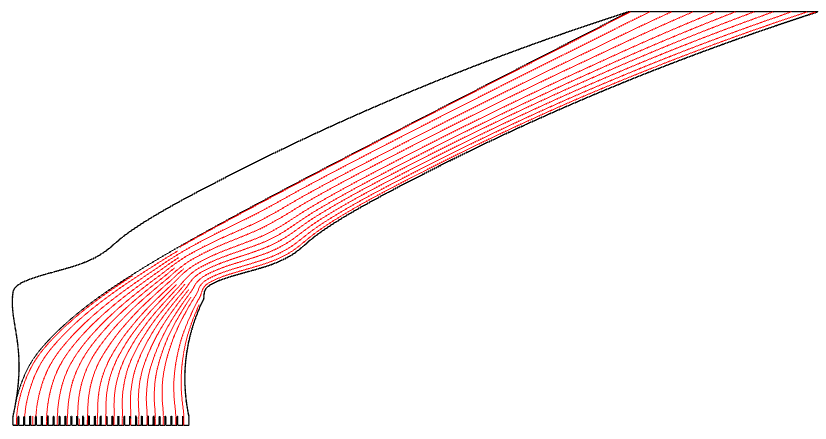
\includegraphics[width=0.55\linewidth, height=5cm, angle=0]{images/HGO_model_geometry/geometry_streamlines.PNG}
    \caption{The outer contours of the epithelial cell with the streamlines that indicate the direction of the keratinous fibers.}
    \label{fig:streamlines}
\end{figure}

\qquad The working principle of the HGO model is also implemented in a simplified square domain. This domain is similar in dimensions as for the models visible in Figure \ref{fig:uniform_elastic_stress}. 





\subsubsection{Model implementation: boundary conditions}\label{sec:HGO_boundary_conditions}
The HGO model is implemented in both the simplified rectangular domain and in the geometry which resembles the epithelial cell. The boundary conditions of the simplified rectangular domain can be found in Section \ref{sec:discrete_model_boundary_con}. The boundary conditions for the geometry resembling the epithelial cell are described in this section and visible in Figure \ref{fig:BC_HGO_model}.\\ 
% These are to some extent equal to the boundary conditions implemented for the simplified geometry with the discrete fibers. 

% beschreven voor het discrete fiber model:
% - Op welke grenzen er welke krachten werken
% - de stijfheid van de individuele componenten
% - geometrische parameters: afstanden tussen fibers en celgrens
% - bonding tussen fibers en matrix materiaal


\begin{figure}[h!]
    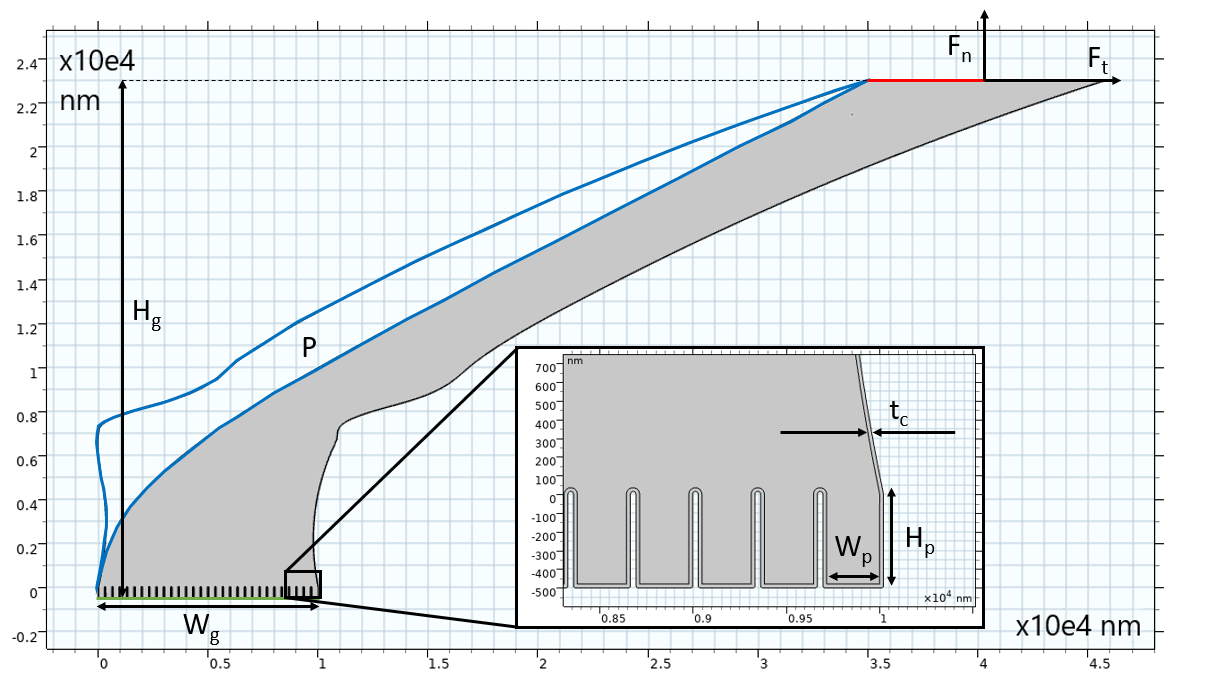
\includegraphics[width=0.9\linewidth, height=8cm, angle=0]{images/HGO_model_geometry/BC_HGO_model.png}
    \caption{The dimensions and boundary conditions of the model which resembles the epithelial cell. The lower boundary is coloured green, the upper boundary is coloured red. The lower boundary is fixed while the external forces $F_{n} \& F_{t}$ are applied on the upper boundary. The blue boundaries enclose the lymph space. The lymph fluid exerts a pressure $P$ on the boundaries of the lymph space. $H_{g}$ and $W_g$ represent the height and base width of the epithelial cell respectively. The epithelial cell is enclosed by a cornified cell layer with thickness $t_{c}$. The epithelial cell has a total of 30 pillars. The height and width of these pillars is represented by $H_{p}$ and $W_{p}$ respectively.}
    \label{fig:BC_HGO_model}
\end{figure}

\qquad The points of attention to be addressed to obtain a mechanical response that matches best with the mechanical behaviour of a real epithelial cell are:
\begin{enumerate}
    \item The lower geometry boundary, highlighted in green in Figure \ref{fig:BC_HGO_model} is fixed. This assumption is also implemented in the simplified rectangular geometry described in Section \ref{sec:discrete_model_boundary_con}. The reasons for the implementation of this condition are the same for the epithelial cell based geometry. % fixed bottom
    \item The upper boundary is loaded with the applied forces $F_{n} \& F_{t}$ these forces resemble the  the perpendicular and tangential loads respectively. This loading configuration is a simplification of the real loading configuration in which the loads would be more evenly distributed over the material domain. % loads on the upper boundary
    \item The boundary conditions on the left and right cell boundaries are necessary to prevent unrealistic deformations in the y-direction. The relatively large distance in the x-direction between the point of application of the forces and the point of application of the reaction force on the base of the epithelial cell can cause a large deformation in the y-direction when a normal force is applied. In reality however, the space under the epithelial cell is filled with other cells which will resist such a large deformation. To resemble the mechanics of the neighbouring cells, the lower boundary is subjected by a force per unit area in the x and y-direction. These parameters are represented by $\sigma_{xx}$ and $\sigma_{yy}$ which are defined as visible in Equation \ref{eq:BC_right}. In these equations the displacement is represented by $u$ and $v$. The parameter $L$ represents an estimate of the maximum displacement and the parameter $E_s$ represents the Young's modulus of the surrounding cellular material. The values of these parameters is $10 \mu m$ and $100 kPa$ respectively. The value of $E_s$ is derived from the indentation experiments performed by Barnes et al. as can be seen in Table \ref{tab:experiments_literature}. % The left and right boundaries
    
    \begin{gather}
        \sigma_{xx} = \frac{-u}{L} E_{s},\nonumber\\
        \sigma_{yy} = \frac{-v}{L} E_{s}
        \label{eq:BC_right}
    \end{gather}
    
    \item The upper boundary of the cell (in red in Figure \ref{fig:BC_HGO_model}) is constrained in rotation. This condition resembles a realistic situation in which concatenated cells will not have full rotational freedom. This condition is also described in Section \ref{sec:discrete_model_boundary_con}. % rigid connector on the upper boundary
    \item The lymph fluid in the domain enclosed by the boundaries visible in blue in Figure \ref{fig:BC_HGO_model} consists mainly out of water which can be assumed an incompressible fluid. Equation \ref{eq:BC_pressure} defines the pressure $P$ on the boundaries of the lymph space as a function of the initial undeformed area $A_{0}$ and the variable area $A$ of the domain. This is a simple and effective way of maintaining a constant volume in an enclosed domain. The surface area of the lymph domain is defined with an integration on the domain borders. The displacement of the lymph fluid is considered irrelevant and therefore excluded. This also saves computational resources. 
    
    \begin{equation}
         P = A - A_{0}
        \label{eq:BC_pressure}
    \end{equation}
    % pressure in the cytoplasm
    \item The mechanical properties implemented for the cornified cellular layer are based on a the assumption that this relatively thin layer(10 nm) has linear elastic properties with a Young's modulus of $100 [MPa]$, a Poisson ratio of $0.4$ and a density of $1000 [kg/m^3]$. These properties bring the mechanical behaviour in the range of other keratinous bio-materials as discussed in Section \ref{sec:bio_material_properties}.   % the properties of the cornified cellular layer
    \item The mechanical properties of the fibrous domain are implemented with the HGO model. This material model requires the constants $k_1$ and $k_2$ which are both associated with the anisotropic contribution of the fibres to the overall response. The stiffness of the fibers is expressed by $k_1$ and $k_2$ represents the amount of fiber non-linearity. This non-linear behaviour is visible in the amount of strain stiffening since the fibres in the implemented model to not have any stiffness in compression. The material stiffness of the base material is represented by the parameter $C_{10}$. Based on the stiffness values described in Section \ref{sec:bio_material_properties}, the true stiffness of the connective tissue is expected to fall in a range of $C_{10} = 1-10 [MPa]$ and the stiffness of the keratin is expected to be the range of $K_1 = 1-10 [GPa]$. Typical values for the parameter $k_2$ are between 0.5 and 5. The first approximation implemented in the model is $k_{2} = 1$. The value of the parameter $k_1$ is varied, this is discussed further in Section \ref{sec:results}.\\ % HGO model constants
\end{enumerate}






\subsubsection{Model validation}\label{sec:HGO_model_validation}
% de validadtie voor het discrete model is als volgt:
% - vergelijking van een blok met linear elastische eigenschappen 
% - met een blok met composiete materiaal eigenschappen
% - dit wort dan weer vergeleken met het model van xue et al.

% in dit gedeelte een geometrie met dunne fibers die dan beter in de buurt moet komen van het HGO model en het HGO model zelf
The HGO model is basically a simplified version of a fiber re-enforced material in which the fibers are relatively thin and everywhere present such that the directional properties of the fibers are present everywhere in the material. For validation of the HGO material model, this model can be compared with the model of Xue et al. as is also described in Section \ref{sec:discrete_model_validation}. 


\begin{figure}[h!]
    \includegraphics[width=0.6\linewidth, height=6cm, angle=0]{images/HGO_model_validation/validatie_matlab_plot.jpg}
    \caption{The $S_{22}$ component of the stress along the length of the geometry for different material models. The models are all loaded with an equal force in the y-direction while the loer boundary of is fixed. The stress response of the uniform linear elastic model and the uniform hyperelastic model are very similar and are added for comparison with the composite material models and the HGO model.}
    \label{fig:HGO_validation}
\end{figure}

The validation of the HGO model is divided in several steps in which the fiber density is increased from a few discrete fibers with finite thickness to an infinite number of infinitely thin fibers. The $S_{22}$ component of the stress response of the different models is visible in Figure \ref{fig:HGO_validation}. 
\begin{enumerate}
    \item The first step of the validation involves the discrete fiber model discussed in Section \ref{sec:discrete_model_validation}. This model involves only a few and relatively thick discrete fibers which are well bounded to the matrix material. The largest magnitude of the stress is visible between the fibers and the contact surface.
    \item The second step in the validation of the HGO model involves a model in which more and thinner fibers are present. In this model is visible that the stress concentrations are still visible at the tips of the fibers. The magnitude of the stress at the tips of the fibers however, is much lower compared to the stresses visible for the coarse fiber model. The mechanical behaviour of the fine fiber model shows that a finer fiber configuration is beneficial for the magnitude of the contact stresses. The stress drops at the edge of the geometry where no fibers are located. 
    \item Based on the stress distribution of the fine fiber model, the stress distribution of the HGO model can be expected to be uniform over the whole length of the domain since the mechanical properties of the fibers are present everywhere in the geometry. The stress response of the HGO model as visible in Figure \ref{fig:HGO_validation} does meet this expectation. This model is set up
    with the parameters $k_{1} = 2 [MPa]$ and $k_{2} = 200 [MPa]$. The difference between the fine fiber model and the HGO is also visible in Figure \ref{fig:HGO_fine_fibers_val}. The largest difference between these two models is visible near the boundary of the geometry. This is mainly caused by the absence of fibers near the boundary of the geometry for the fine fiber model. The peaks of the HGO model near the right edge of the boundary are caused by numerical instability and will be further discussed in Section \ref{sec:HGO_model_sensitivities}. 
\end{enumerate}

\begin{figure}[h!]
\includegraphics[width=0.6\linewidth, height=3.5cm, angle=0]{images/HGO_model_validation/validatie_HGO_en_fine_fibers.jpg}
\caption{Difference between the HGO model and the fine fiber model.}
\label{fig:HGO_fine_fibers_val}
\end{figure}

% nog even over de validatie, is het goed genoeg?
\qquad The modelling results discussed above validate the use of the HGO model for a geometry which would otherwise be filled with fine fibers. The validation described above however, only validates the HGO model for a configuration in which the load is applied in the direction of the fibers. Therefore, this validation needs to be elaborated to investigate the validity of the HGO model for a case in which the geometry is not loaded in the direction of the fibers.\\


\qquad Figure \ref{fig:HGO_validation_1} shows the $S_{22}$ stress component in an simplified geometry that is loaded with a force in the x-direction(perpendicular to the direction of the fibers) and with a force in the y-direction. The stress values of the models loaded in tension are comparable with the stress values visible in Figure \ref{fig:HGO_validation}. The model results of the models loaded with a normal and a shearing force show that a shearing force significantly increases the stress in the geometry. This increase in stress is also visible for the $S_{11}$ stress component. The $S_{13}$ component is zero along the whole length of the lower geometry boundary. Figure \ref{fig:HGO_validation_1} shows the stress in the lower left corner of the geometry while the same effects in the stress response can also be observed in the lower right corner.\\  

\begin{figure}[h!]
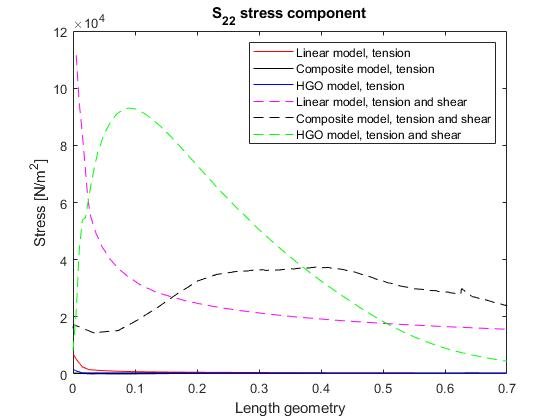
\includegraphics[width=0.7\linewidth, height=6.5cm, angle=0]{images/HGO_model_validation/comparison_all_data.jpg}
\caption{Stress response of the linear model, the fine fiber and the HGO model for different loading configurations.}
\label{fig:HGO_validation_1}
\end{figure}

\qquad The difference between the stress distribution for the HGO model and the composite model increases with the introduction of the shear force. When loading a geometry like the geometry visible in Figure \ref{fig:uniform_elastic_stress} with a force in the x-direction while the bottom is fixed, a bending moment is created. This bending moment introduces reaction forces in the y-direction from which the magnitude and forces are dependent on the location in the geometry. These reaction forces are the largest at the right and left boundaries of the geometry. This is also visible in the $S_{11}$ and $S_{22}$ stress components which are the largest near the lower right and left corners of the geometry. The forces in the x-direction are the sum of the shear forces and the forces induced via the deformations caused by the forces in the y-direction. This second component is dependent on the constant value of the Poison ratio.\\ 


\qquad Figure \ref{fig:HGO_validation_2} shows the these stress components for a rectangular geometry with the same dimensions as visible in Figure \ref{fig:uniform_elastic_stress}. This geometry is fixed at the lower boundary and the right boundary is loaded with a force in the x-direction. In these figures it is visible that:

\begin{enumerate}
    \item In the right subplot of Figure \ref{fig:HGO_shear_S22} is visible that the $S_{22}$ component for the HGO model when loaded in compression and in shear is very similar to this component for the linear model. This can be explained by the absence of directional dependent properties for the HGO model when loaded in compression. Without these directional dependent properties, the HGO model acts as a pure solid with a Neo-hookean material model. The stress response of a solid geometry with a Neo-hookean material model is very similar to the response of a linear elastic material model for the boundary and loading conditions used in this validation simulation.
    \item In the left subplot of \ref{fig:HGO_shear_S22} is visible that the different variations of the HGO model do have a stress peak in the left corner of the geometry. This stress peak is most probably caused by the strain stiffening properties of the HGO model. This effect can be expected at the left corner of the geometry due to the reaction forces implied by the imposed moment which are in the direction of the strain stiffening material model properties.  
    \item The $S_{11}$ component visible in the corners of the geometry visible in both subplots of Figure \ref{fig:HGO_shear_S11} follows the deformation that is caused by the $S_{22}$ component. The deformation at the very left edge is relatively low due to the strain stiffening effect discussed above. This is most probable the reasons why the peak of the $S_{11}$ component occurs right before the left edge of the geometry as visible in the left subplot of Figure \ref{fig:HGO_shear_S11}. 
    \item The stress components of the linear composite model in the left corner of the geometry visible in the left subplots of Figure \ref{fig:HGO_shear_S11} \& \ref{fig:HGO_shear_S22} are much lower than the stresses found for the other material models. The main reasons for this is most probable caused by the buffering nature of the complient material situated at the edge of the geometry for the discrete fiber model geometry. The strain at the edges of the linear composite model is visible in Figure \ref{fig:i4_invariant}. This invariant can be calculated with Equation \ref{eq:I4_short} and represents the strain in the direction of the fibers. In Figure \ref{fig:i4_invariant} is visible that the linear composite model has more strain at the edges than the HGO model. This strain however, does not result in a higher values for the $S_{11}$ and $S_{22}$ stress components because of the buffering nature of the outer compliant layer present at the edge of the composite linear model. The relatively low strain for the HGO model can be explained with the strain stiffening effect. 
    \item The strain stiffening composite model is similar to the linear composite model but has fibers that display non-linear strain stiffening behaviour. This strain stiffening behaviour is also discussed for other bio-materials \cite{holzapfel2000new}. The mechanical properties of these fibers are similar to these of the HGO model with $C = e$ used in Equation \ref{eq:w4_var}. The $S_{11}$ and $S_{22}$ components found for the strain stiffening composite model display that the strain stiffening leads to a higher stress at the top of the fibers as visible in the left subplots of Figure \ref{fig:HGO_shear_S11} \& \ref{fig:HGO_shear_S22}. The directional dependence of the strain stiffening properties however, leads to higher values for the $S_{11}$ and $S_{22}$ components in the right corner of the geometry as visible in the right subplots of Figure \ref{fig:HGO_shear_S11} \& \ref{fig:HGO_shear_S22}. It is visible for this model that the buffering nature of the complient layer at the left edge of geometry prevents the development of stresses. This effect is also described for the linear composite model, but on both edges. 
\end{enumerate}


\begin{figure}[h!]
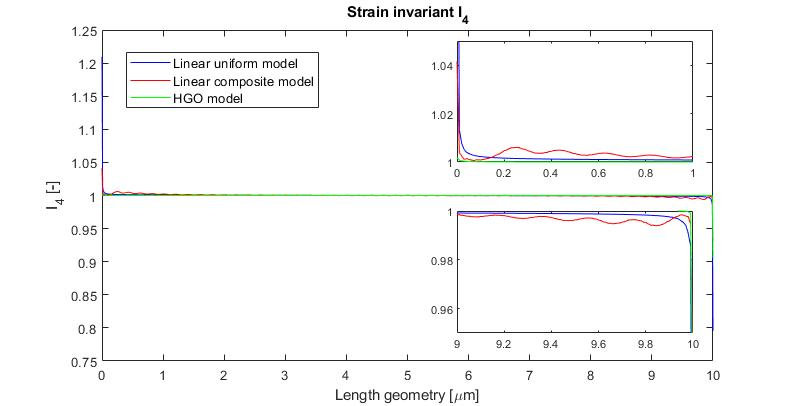
\includegraphics[width=0.7\linewidth, height=6.5cm, angle=0]{images/HGO_model_validation/Invariant_i4.jpg}
\caption{Strain invariant for different material models. The invariant has a value of one for zero strain conditions.}
\label{fig:i4_invariant}
\end{figure}


% nog goed naar het composite lineare model kijken!
%  - wat als het composite model niet lineaire eigenschappen heeft?
%  - geen significante verandering voor niet lineare eigenschappen van het composiet lineare model


%hier nog verder gaan over de strain stiffening properties 
\qquad The $S_{11}$ and $S_{22}$ stress components visible in Figure \ref{fig:HGO_shear_S11} \& \ref{fig:HGO_shear_S22} are plotted for three variants of the HGO model to provide insight in the strain stiffening properties of the HGO model. The strain stiffening behaviour of this model is determined by Equation \ref{eq:anisotropic_w4}. This equation can also be written as visible in Equation \ref{eq:w4_var}. The effects of varying the parameter $C$ are visible in Figure \ref{fig:HGO_shear_S11} \& \ref{fig:HGO_shear_S22}. As is visible in this figure, the stress in the x-direction can be brought closer to the response of the fibrous model by tuning the exponential function that determines the $W_{4}$ component of the HGO model.\\ 

\begin{equation}
    W_4 = \frac{k_1}{2k_2}(C^{k_2(I_4 - 1)^2} - 1)(I_{4}>1)
    \label{eq:w4_var}
\end{equation}

\qquad The reduction of the peak magnitude of the $S_{11}$ component is most probably caused by the decreased strain at the locations where the strain stiffening occurs. The $S_{22}$ component of the stress in these locations does not match the response of the fibrous model. The slope of this component however, is affected by the tuning of the parameter $C$ as visible in left subplot of Figure \ref{fig:HGO_shear_S22}.\\

\qquad The tuning of the $W_{4}$ component of the HGO model gives the best results for the default value $e$ for the parameter $C$. Values higher or lower than $e$ give a worse result in therms of the stress peak visible in the left subplot of Figure \ref{fig:HGO_shear_S11}. The maximum value of the $S_{22}$ component visible in the left and right subplot of Figure \ref{fig:HGO_shear_S22} is the lowest for the smallest value for $C$. This can be explained by the reduced effect of the strain stiffening for this value. The magnitude of $C$ therefore determines the ratio of the $S_{11}$ and $S_{22}$ components.\\ 

\begin{figure}[h!]
    \begin{subfigure}{0.95\textwidth}
    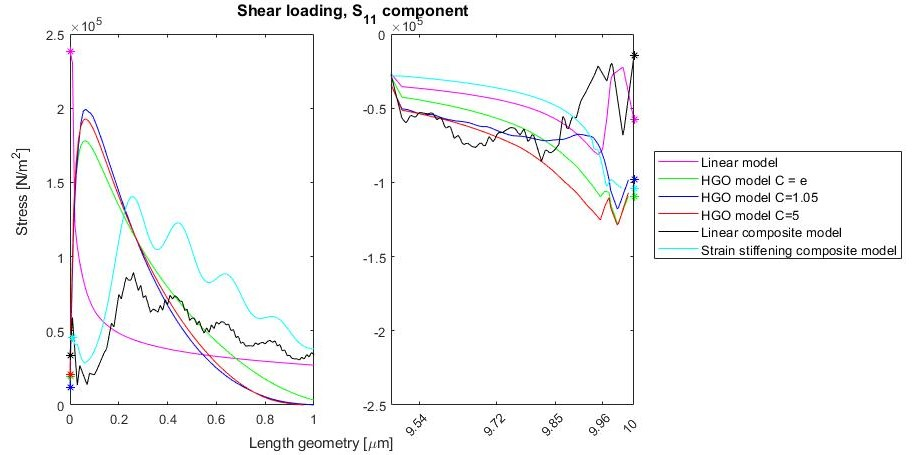
\includegraphics[width=\textwidth, height=7cm, angle=0]{images/HGO_model_validation/HGO_model_shear_S11.jpg}
    \caption{}
    \label{fig:HGO_shear_S11}
    \end{subfigure}
    \hfill
    \begin{subfigure}{0.95\textwidth}
    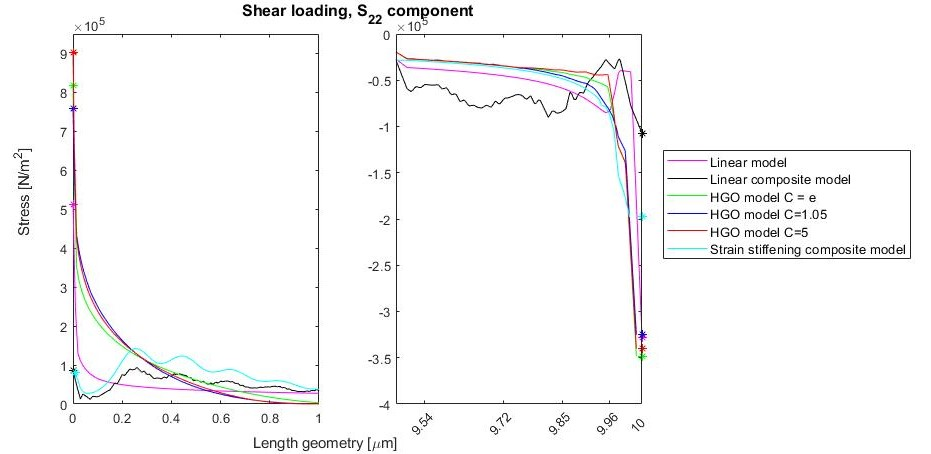
\includegraphics[width=\textwidth, height=7cm, angle=0]{images/HGO_model_validation/HGO_model_shear_S22.jpg}
    \caption{}
    \label{fig:HGO_shear_S22}
    \end{subfigure}
    \caption{The $S_{11}$ and $S_{22}$ stress components in the x-direction and y-direction for a shear loaded configuration of the simplified HGO model. The asterisks at the start and the end of the curves mark the value of the stress components at the outer edges of the geometry.}
    \label{fig:HGO_validation_2}
\end{figure}

\qquad The observations in this section point out that the HGO model differs from the discrete fiber model when the load on the geometry causes a non-uniform distribution of forces along the interface between the geometry and the substrate. This is caused by the strain stiffening of the HGO model and the buffering nature of the compliant material present along the edges of the composite material model.\\ 

\qquad Modelling a complex geometry with a large number of mesh elements as is visible in Figure \ref{fig:geometry_solidworks} requires a material model in which individual fibers are not present. The HGO model meets this requirement. This model however does differ from the (strain stiffening) composite model as discussed above. These differences are taken into account when discussing the modelling results of the model that incorporates the geometry visible in Figure \ref{fig:geometry_solidworks}.\\




% hier redenen bedenken..kan het het nog dichterbij gebracht worden en kan de sensitivity analysis hier bij helpen?





\subsubsection{Model sensitivities}\label{sec:HGO_model_sensitivities}
% In order to tune the HGO model as good as possible to the expected material properties of the tree frog, the parameters $c_10$, $k_1$ and $k_2$ are varied to evaluate their influence on the HGO model behaviour. The HGO model is again implemented for a rectangular domain with the same dimensions as used for the validation step and the forces and boundary conditions applied are the same as described for Figure \ref{fig:test_geometry}.\\ 

% Variations of the parameter $k_2$ while the other parameter are kept constant do not change the stresses in the material. The parameter $k_2$ does only effect the strain stiffening behaviour of the model. therefore, it only effects the amount of deformation of the model, in particular the strain of the geometry caused by the $S_{22}$ component of the stress. 

% The parameters the stiffness of the base material and fibrous component is described by respectively $c_M$ and $k_1$. The influence of the value of these two parameters is investigated by varying these parameters with respect to each other by varying $k_1$ while keeping $c_M$ at a constant value. The value of $k_1$ is given by the relation $k_1 = c_M R$ with $R$ representing the ratio between $c_M$ and $k_1$. The deformation and stress for $R = 100$ are visible in Figure \ref{fig:tuning_deformation}. In this figure is visible that the highest stresses occur at the lower left corner of the geometry. 

% \begin{figure}[h!]
%     \includegraphics[width=\linewidth, height=6cm, angle=0]{Pictures/tuning/deformation.png}
%     \caption{Deformation of the domain and visualization of the $S_{22}$ stress component.}
%     \label{fig:tuning_deformation}
% \end{figure}

% Figure \ref{fig:tuning_11_com} and \ref{fig:tuning_22_com} show that the $S_{11}$ and the $S_{22}$ components are both influenced bu the value of the parameter $R$. For high values of $R$ the stress in the lower left corner of the geometry reaches significantly higher values than for lower values for this parameter. 

% \begin{figure}[h!]
%     \centering
%   \subfloat[\label{fig:tuning_11_com}]{%
%       \includegraphics[width=\linewidth, height=6.5cm, angle=0]{Pictures/tuning/stress_11_var_cmk1.jpg}}
%     \hfill
%   \subfloat[\label{fig:tuning_22_com}]{%
%         \includegraphics[width=\linewidth, height=6.5cm, angle=0]{Pictures/tuning/stress_22_var_cmk1.jpg}}
%   \caption{Stress component $S_{11}$ and $S_{22}$ for various values of the ratio between the HGO model parameters $c_M$ and $k_1$. The x-axis has a logarithmic scale to visualize the stress at the left edge of the geometry.}
% \end{figure}
% \subsubsection{Solver configuration}
%  the model involves non-linear behaviour which can sometimes lead to convergence issues. The measures taken to prevent convergnece issues and to shorten computation time are as follows:
%  - the estimates of the initial values of the dependent values need to be chosen carefully. Comsol uses these values as an estimate for the computional result and therefore benefits from an accurate prediction of these values. 
 
%   % question:
%  % why is the model more computational intensive for a larger ratio between Cm and k1?
%  Although the properties of the HGO model are already compared with the model using by Xue et al., it still makes sense to investigate if the introduction of a shear force force does effect the model performance. Figure \ref{fig:validation_shear} shows the absolute value of an average stress in the geometry when this geometry is loaded with both shear and a perpendicular load. This average value is composed of the stress components $S_{11}$ and $S_{22}$ represented by Equation \ref{eq:average_stress}. The $S_{13}$ component is zero along the whole length of the lower geometry boundary and is therefore not taken into account. The stress values represented with the continuous lines are comparable with the values visible in Figure \ref{fig:HGO_and_fine_fibers} while the dotted lines represent the model results for a model which also includes a shearing force. This additional shearing force significantly increases the stress in the geometry. The difference between the stress distribution for the HGO model and the composite model increases with the introduction of the shear force. This can be caused by...% hier redenen bedenken..kan het het nog dichterbij gebracht worden en kan de sensitivity analysis hier bij helpen?
 
 
 
 
 
 
\subsubsection{Data processing}




\section{Experimental setup}


\begin{table}[h!]
    \centering
    \begin{tabular}{|l|c|c|c|}\hline
    \diaghead{\theadfont Diag ColumnmnHead}%
    {Stiffness PDMS}{Fiber thickness}&
    \thead{Reference,\\no inserted fibers} & \thead{Thin fibers} & \thead{Coarse fibers}\\ 
    \hline
    $1 [MPa]$ & I & II & III \\    
    \hline
    $3 [MPa]$ & IV & V & VI \\    
    \hline
    \end{tabular}
    \caption{Different test pieces fabricated}
    \label{tab:experimental_variants}
\end{table}


\subsection{Modelling}
% het tweede orde ogden model is gevonden als het beste om hyperelastisch materiaalgedrag van PDMS te modelleren. De parameters zijn gefit in het artikel van Kim et al. \cite{kim2011measurement}
  
%   de parameter zijn $\mu_1 = 63.49$ [MPa] en $\mu_2 = 0.041$ [MPa] met $\alpha_1 = 	6.371e-10$ en $\alpha_2 = 3.81166$ en een bulk modulus van $962$ [MPa] voor een mengverhouding van basis polymeer en curing agent van 1:10. The density of PDMS is $965 [kg/m^3]$.
  
  
%   het tweede orde ogden model is gevonden als het beste om hyperelastisch materiaalgedrag van PDMS te modelleren. De parameters zijn gefit in het artikel van Kim et al. \cite{kim2011measurement}
% de parameter zijn $\mu_1 = 63.49$ [MPa] en $\mu_2 = 0.041$ [MPa] met $\alpha_1 = 	6.371e-10$ en $\alpha_2 = 3.81166$ en een bulk modulus van $962$ [MPa] voor een mengverhouding van basis polymeer en curing agent van 1:10. The density of PDMS is $965 [kg/m^3]$.
\subsection{Fabrication}
\subsection{measurement setup}
\subsection{Boundary conditions}
\subsection{Data processing}
\chapter{Results}\label{ch:results}

\section{modelling}
% hier steeds het discrete model en het HGO model vergelijken! dit is niet overal toepasbaar maar als het toepasbaar is, is dit wel de beste structuur om ook gelijk de verschillen inzichtelijk te maken tussen de twee modellen

\subsection{Influence fiber bonding}\label{sec:results_fiber_bonding}
\subsection{Influence force direction}\label{sec:results_force_direction}
Matching the magnitude of the normal and tangential force components is also described by...
\subsection{Behavioral adaptions}\label{sec:results_behavioral_adaptions}
\subsection{Influence fiber stiffness}\label{sec:results_fiber_stiffness}
\subsection{Influence fiber density}\label{sec:results_fiber_density}
\subsection{}\label{sec:results_}
\subsection{}\label{sec:results_}
\subsection{}\label{sec:results_}









% - De krachten die ook daadwerkelijk op de kikker staan nemen en kijken welke contactkrachten dit oplevert 
% % dit nog doen!
% - vervolgens checken of deze krachten laag genoeg zouden zijn om ahesie te behouden uitgaande van capilaire adhesie met hondert procent contactoppervlak




% The results of the model visible in Figure \ref{fig:coarse_fibers} clearly show that the stress is strongly influenced by the location of the fiber re-enforcement. This is also visible for the results of the model with the small fibers but the variation in stress is much less for this model. The most important observation is that both fibre re-enforced models have a much lower value for the stress at the end of the geometry at $L = 10 \mu m$ on the horizontal axis. This reduction in peak stress increases the adhesive strength of the material. 

% \begin{figure}[h!]
%     \includegraphics[width=\linewidth, height=6cm, angle=0]{Pictures/validation/validatie_matlab_plot.jpg}
%     \caption{Stress in the different models used for the validation. The average stress is equal for all the models.}
%     \label{fig:matlab_validation_stress}
% \end{figure}


% \section{Experimental testing}

% \begin{figure}[h!]
%     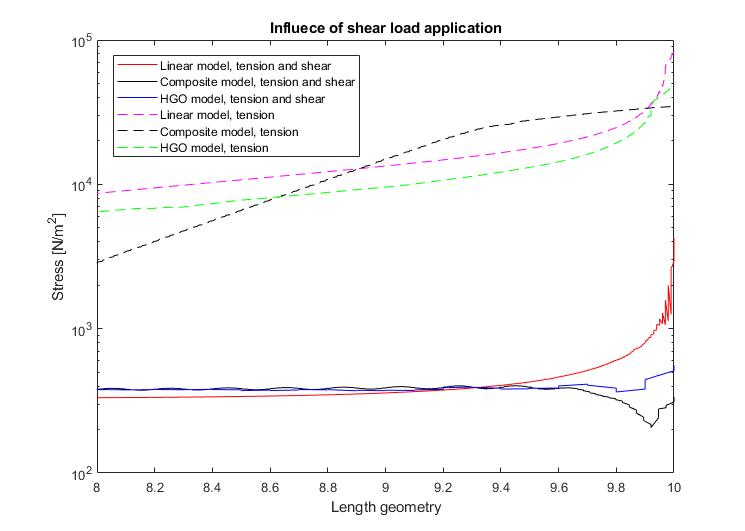
\includegraphics[width=\linewidth, height=6cm, angle=0]{Pictures/validation/comparison_all_data.jpg}
%     \caption{Stress in the contact surface for a geometry loaded with a shear force and a perpendicular force. The x-axis represents the corner of the geometry which is the location of the relevant material behaviour.}
%     \label{fig:validation_shear}
% \end{figure}



% \begin{figure}[h!]
%     \includegraphics[width=\linewidth, height=6cm, angle=0]{Pictures/validation/test_geometry_boundaries.png}
%     \caption{Simple geometry for model testing and validation. The upper red boundary is subjected to the shear  and perpendicular forces which are represented by $F_t$ and $F_n$ respectively. The lower blue boundary is fixed and the green side boundaries are free. Stress measurements are performed on the blue boundary.}
%     \label{fig:test_geometry}
% \end{figure}
\chapter{Discussion}\label{ch:discussion}


% % over de proximal pulling: kijk maar even wat hier van waar is...
% The limb spreading of the frog however does also significantly increase the x-component of the proximal pulling force. This is clearly visible in Figure \ref{fig:limb_spreading_second_spread}. The frog does spread all its limbs but the effect of the spreading is most pronounced for the hind limbs since these are much longer than the front limbs. The frog can also exert a higher proximal pulling force with the hind limbs since these are also much stronger than the front limbs. In Figure \ref{fig:frog_feet_streched} the forces involved are made visible. This sketch assumes a situation in which the magnitude of the pulling forces on the front limbs is smaller than the magnitude of the pulling forces on the hind limbs. This difference is caused by the increase in the x-component $F_{p,1_x}$ of the pulling force on the lower limbs $F_{p,1}$. 




% When adding the x-components of the proximal forces to the equations to the Matlab model we assume that the frog is exerting an increased x-component of the proximal pulling force when more more adhesion is needed to stay to the surface. An increase of the proximal force increases the the tangential forces while the normal forces are not affected since $F_{n,1}$ and $F_{n,2}$ are not dependent on the tangential force components. The frog can thus match the curve of the required normal forces for adhesion with a similar increase in the tangential force. This is visible in Figure \ref{fig:matching_forces}. The results visible in this figure are produced under the assumption that the tree frog performs its first spread when the angle $\theta$ of the surface the frog is attached to has a value of $\frac{\pi}{3}$. The second spread occurs at $\theta = \frac{2\pi}{3}$. 


% % Especially the parameter related to large strain stiffening (k2) increased with loading rate %dit gaat over tijds-afhankelijk gedrag!


% % over het model met de kikker op de draaitafel
% These values are purely imposed by the gravitational force on tree frog adhered to a vertical surface. However, there are reports that describe much higher loading of the adhesive pads of the tree frog. Bijma et al. reported that the frog species \textit{Trachycephalus resinifictrix} can handle loads up toe  14.4 times the body weight with a single digital pad during a landing after a leap \cite{bijma2016landing}. 


% wat is de invloed van de rigid connector? beschrijf hierin het verschil tussen het model van de epitheelstructuur met de rigid connector en de geteste situatie waar deze niet inzit!



% % over de stijfheid parameters geimplementeerd in het HGO model:
% \qquad These stiffness values are significantly higher than the values used by others that use the HGO method to model the mechanical properties of bio-materials. In the work of Holzapfel et al. the mechanical properties of mouse blood vessels are modelled using the values $k_1 = 4-40 [kPa]$, $k_2 = 0.5 - 5$ and $C_{10} = 26 [kPa]$ \cite{collins2011mechanical,holzapfel2000new}. The mechanical properties of the adhesive structure of the tree frog however, are expected to be dominated by the presence of keratin and not collagen. The stiffness of the individual components and the extend to which these components are present in the epithelial cells is discussed in Section \ref{sec:bio_material_properties} and visible in Figure \ref{fig:epithelial_cell_components}. 


% % hier verder
% The HGO model shows a slightly different stress distribution than the other models. The HGO model does not incorporate discrete fibers which results in a more even stress distribution along the contact surface. The largest difference between the HGO model and the fine fiber model is at $L = 10 \mu m$. This difference is however much less than the difference between the HGO model and the coarse fiber model and is expected to reduce further for a higher fiber density for the discrete fiber model. Figure \ref{fig:HGO_and_fine_fibers} shows the stresses of the HGO model, the fine fiber model and the difference between these models.

% \begin{figure}[h!]
%     \includegraphics[width=\linewidth, height=3cm, angle=0]{Pictures/validation/validatie_HGO_en_fine_fibers.jpg}
%     \caption{Stress in the HGO model and the fine finer model and the difference between these.}
%     \label{fig:HGO_and_fine_fibers}
% \end{figure}



% de krachtenverdeling wordrt bepaald door de verhouding tussen W1 en W4. dit zijn de isochoric strain energy densities. 

% the isochoric strain energy density relates the strain energy density to the deformation geradient. 

% for normal hyperelastiv materials Comsol computes the second piola kirchhoff stress as 

% \begin{equation}
%     S = 2\frac{\delta W_s}{\delta C}
% \end{equation}

% with W for the strain energy density and C for the right gachy green deformation tensor. 

% for isochoric materials(with a constant volume) a weak constraint is added in the form of $J_{el} = 1$ the auxiliary pressure variable acts as a lagrange multiplier to enforce this constaint. The eqaution for the piola kirchhoff stress is than defined as follows:

% \begin{equation}
%     S =  -p_{w}JC^{-1} + 2\frac{\delta W_{iso}}{\delta C}
% \end{equation}

% $W_{1}$ and $W_{4}$ are both isochoric components. The difference is in the domain they represent. $W_1$ is for the isotropic material properties and $W_4$ is for the anisotropic material properties. 

% Strain for both components is the same for the same location. The ratio between $W_1$ and $W_4$ however is different when the ratio between Cm and k1 is varied. 



% Strain stiffening is iets dat hoort bij de materialen die in de natuur voorkomen, hier nog wel bronnen bij vermelden! hiervoor kun je terugverwijzen naar de vorige onderdelen. De effecten die hier door strain stiffning geintroduceerd worden kunnen dus zeker heel reel zijn


% niet linear gedrag met strain stiffening is gematcht aan het HGO model door Holzapfel et al \cite{holzapfel2000new}

\chapter{Conclusion}\label{ch:conclusion}



%\input{chapters/Appendix_A.tex}
%\bibliography{report}

%\addcontentsline{toc}{chapter}{Bibliography}
%\chapter*{Bibliography}
\printbibliography

% \newrefcontext[sorting=none]
% \begingroup
% \let\clearpage\relax
% \printbibliography[heading=subbibliography, type=book, title={{Books}}] 
% \endgroup
% \newrefcontext[sorting= none]
% \begingroup
% \let\clearpage\relax
% \printbibliography[heading=subbibliography, type=article, title={{Reports, Theses and Individual Papers}}]
% \endgroup
% \newrefcontext[sorting=none]
% \begingroup
% \let\clearpage\relax
% \printbibliography[heading=subbibliography,  type=misc, title={{Electronic Publications}}]
% \endgroup
% \restoregeometry


%% Use letters for the chapter numbers of the appendices.
\appendix
%\input{chapters/Appendix_A.tex}
\end{document}
